\documentclass[aps,pra,12pt,notitlepage,tightenlines]{revtex4-1}
%\usepackage[margin=2.5cm]{geometry}
\usepackage{amsmath,amssymb,textcomp,graphicx,url,bm,lipsum,hyperref,color,subcaption,afterpage,gensymb,
array}

\newcommand\matr[1]{\bm{#1}}
\newcommand\barparen[1]{\overset{\textbf{\fontsize{5pt}{5pt}\selectfont(---)}}{#1}}

\graphicspath{{Images/}}

\newcommand{\nue}{$\nu_e$}
\newcommand{\anue}{$\bar\nu_e$}
\newcommand{\numu}{$\nu_\mu$}
\newcommand{\anumu}{$\bar\nu_\mu$}

\setcounter{totalnumber}{1}

\begin{document}

\title{Upgrading the Near Detector of T2K and Electron \mbox{(Anti-)Neutrino} Detection in a Neutrino Beam \vspace{0mm}}
\author{Wilf Shorrock\vspace{1mm}}
\affiliation{Imperial College London\vspace{-0.5mm}}
\date{June 30, 2018}
\begin{abstract}
\linespread{0.97}
\vspace{1mm} In 2020, the Tokai-to-Kamioka (T2K) experiment is set to enter a new phase of data-taking with a more intense neutrino beam. To make full use of the higher statistics and reduce systematic uncertainties, upgrades to the one of the near detectors---ND280---have been proposed. In this report, the physics of neutrino oscillations are explained and an outline of the T2K experiment is given. The sub-detectors currently comprising ND280 and the structure of its software is described, as well as proposed upgrades. A beam test performed at CERN in June 2018 for the prototype of the new Super-fine-grained detector (Super-FGD), to be installed in the upgraded ND280, is also detailed. A rough plan of the future work the author will undertake is given at the end of the report, which includes analysis of ND280 data for electron neutrino and anti-neutrino interactions in the neutrino beam.
\end{abstract}

\maketitle

\newpage
\tableofcontents
\newpage

\vspace{-8mm}

\section{Introduction}
%In their 1956 paper announcing the discovery of the neutrino, Reines and Cowan stated:
%\begin{quotation}
% ``Each new discovery of natural science broadens our knowledge and deepens our understanding of the    physical universe; but at times these advances raise new and even more fundamental questions than those     which they answer~\cite{1956Natur.178..446R}.''
%\end{quotation}
%At the time, they were referring to the observation of beta decay and how it led to the proposal of the neutrino, but it is rather fitting that we can also apply this statement to the neutrino itself. Since the observation of atmospheric neutrino oscillations at Super-Kamiokande (SK) in the 1990s, a whole new area of research has opened up, and results from further experiments observing reactor neutrinos~\cite{PhysRevLett.108.171803, PhysRevLett.108.191802, PhysRevLett.108.131801} have shown that neutrinos oscillate between three flavour states via three mass eigenstates.

The imprint neutrinos leave on our world is almost unnoticeable due to their vanishingly small cross-sections with respect to everyday baryonic matter. Yet, the ethereal nature of the neutrino belies its importance in the Universe. Neutrinos have pervaded our world almost since the very beginning and they have affected the evolution of entire galactic systems. This is why physicists are persevering in their attempts to measure the properties of the almost undetectable neutrino, a study in which they have made notable progress over the past few decades. 

Since the neutrino was first discovered in 1956 by Reines and Cowan~\cite{1956Natur.178..446R}, the way in which it has been perceived by the scientific community has evolved significantly. After initially thinking all neutrinos were identical, we now know they come in three different flavours: electron, muon and tau neutrinos. Each flavour contributes a lepton number of +1 or $-1$ for its corresponding lepton flavour in all the interactions they participate in, albeit they are extremely rare interactions. The notion of neutrinos having mass is also a new concept, with the neutrino thought of as massless before it was discovered that neutrinos could oscillate in flavour, which is partly credited to the flavour change in atmospheric neutrinos observed by the Super-Kamiokande (SK) water Cherenkov detector in the 1990s~\cite{Fukuda1998}. This effect implies that neutrinos must have some mass, although to have been unmeasured thus far it has to be extremely small, as explained in Sec.\ \ref{sec:osc} of this report.

%Neutrino oscillation has become one of the more promising avenues towards Beyond Standard Model physics. It also helps to shed light on previously unexplained measurements, for example the lack of electron neutrinos originating from the Sun~\cite{PhysRevLett.89.011301}. 

There are several experiments measuring oscillation parameters using neutrinos produced in nuclear reactors, such as KamLAND, Daya Bay, and Double CHOOZ~\cite{Suzuki2014, PhysRevLett.108.171803, PhysRevLett.108.131801}. There are also experiments using neutrino beams produced using particle accelerators. The goals of these latter experiments are to make more precise measurements of the oscillation parameters and to ascertain whether charge parity (CP) is conserved or not.

Tokai to Kamioka (T2K) is an experiment that measures neutrino oscillations over a long distance. It studies neutrinos produced by a proton accelerator. Since it began taking data in 2010, T2K has made precision measurements of the neutrino squared mass splittings and several mixing angles, including one of the first measurements of the mixing angle $\theta_{13}$ (these parameters are explained in Sec.\ \ref{sec:osc})~\cite{PhysRevD.88.032002}. The latest analysis results were published in 2017~\cite{Abe:2017bay}. Over the next few years, the experiment aims to observe CP violation (CPV) in neutrino oscillations with at least a 3$\sigma$ statistical significance (if the CPV is maximal) and discover whether the mixing angle $\theta_{23}$ is maximal, as current measurements suggest. The new phase of the experiment is called T2K-II and will require several upgrades to the experiment's detectors.

This report provides an overview of the proposed upgrades to the T2K experiment's off-axis near detector, ND280. It also gives a description of the beam test carried out with the prototype of one of the new sub-detectors, called the Super-FGD. This description will include a calibration measurement for the detector's photosensors and initial data readings from the beam test. The final section of the report will address my future work, such as the continued development of the ND280 software and an analysis of ND280 data using a new neutrino generator production. Firstly, the theory behind neutrino oscillation will be given, leading on to an overview of the T2K experiment and details on the current state of ND280 and its software.

\section{Neutrino Oscillation Model}
\label{sec:osc}
For neutrino oscillations to exist, the neutrino flavour eigenstates, $(\nu_e, \nu_\mu, \nu_\tau)$, must be different to the neutrino mass eigenstates, $(\nu_1, \nu_2, \nu_3)$. In fact, it must be the case that the flavour eigenstates are coherent superpositions of the mass eigenstates. Hence, they can be equated using the equation
\begin{gather}
\label{eq:pmns}
 \begin{pmatrix}
 \nu_e \\
 \nu_\mu \\
 \nu_\tau 
 \end{pmatrix}
 =
 \begin{bmatrix}
 U_{e1} & U_{e2} & U_{e3} \\
 U_{\mu1} & U_{\mu2} & U_{\mu3} \\
 U_{\tau1} & U_{\tau2} & U_{\tau3}
 \end{bmatrix}
 \begin{pmatrix}
  \nu_1 \\
 \nu_2 \\
 \nu_3 
 \end{pmatrix}
 ,
\end{gather}
where the matrix enclosed by square brackets is the Pontecorvo-Maki-Nakagawa-Sakata (PMNS) matrix, $\matr{U}$ \cite{Maki1962, Pontecorvo1957}. The matrix elements $U_{\alpha i}$ represent the mixing amplitudes of mass state $i$ contained within flavour state $\nu_\alpha$.

$\matr{U}$ is a unitary matrix, so it can be parametrised using three real angles, $(\theta_{12}, \theta_{13}, \theta_{23})$, and a real phase, $\delta_\mathrm{CP}$, to give
\begin{gather}
 \matr{U} = 
 \begin{bmatrix}
 1 & 0 & 0 \\
 0 & C_{23} & S_{23} \\
 0 & -S_{23} & C_{23}
 \end{bmatrix}
 \begin{bmatrix}
 C_{13} & 0 & S_{13}e^{-i\delta_\mathrm{CP}} \\
 0 & 1 & 0 \\
 -S_{13}e^{i\delta_\mathrm{CP}} & 0 & C_{13}
 \end{bmatrix}
 \begin{bmatrix}
 C_{12} & S_{12} & 0 \\
 -S_{12} & C_{12} & 0 \\
 0 & 0 & 1
 \end{bmatrix}
 ,
\end{gather}
where $C_{ij} = \cos\theta_{ij}$ and $S_{ij} = \sin\theta_{ij}$. These mixing angles and phases are what oscillation experiments measure. A non-zero value of the $\delta_{CP}$ phase (given that $S_{13}\neq 0)$ would mean that neutrino oscillations are CP-violating. There may be two extra phase parameters required if neutrinos are Majorana particles (Majorana particles are their own anti-particles) but these have no effect on oscillation measurements, assuming the neutrino's right-handed counterpart is extremely massive, which is likely seeing as the neutrino itself is so light~\cite{Kayser:2005cd}.

Eq.\ \eqref{eq:pmns} encapsulates much of the physics behind neutrino oscillations. It implies that, following the weak decay $W \rightarrow l_\alpha\nu_\alpha$, where $\nu_\alpha$ is a neutrino flavour eigenstate and $l_\alpha$ is the corresponding charged lepton state with flavour $\alpha$, the neutrino will propagate as a mixture of the mass eigenstates that interfere quantum mechanically. This means the probability of the neutrino's flavour, when measured, is dependent on the distance the neutrino travelled~\cite{Kayser:2005cd}. 

For a detailed derivation of the neutrino oscillation probabilities, see Kayser~\cite{Kayser:2011jn}. Here, only the end result is quoted, which is the probability of a \mbox{(anti-)neutrino} with initial flavour $\alpha$ and energy $E_\nu$ propagating a distance $L$ and being detected with flavour $\beta$:
\begin{align}
\label{eq:p}
P\Big(\barparen{\nu_\alpha}\rightarrow\barparen{\nu_\beta}\Big) = \delta_{\alpha\beta}&-4\sum^3_{i<j}\Re[U_{\alpha i}U_{\beta i}^*U_{\alpha j}^*U_{\beta j}]\sin^2\bigg(\Delta m^2_{ij}\frac{L}{4E_\nu}\bigg) \notag \\
& \mp 2\sum^3_{i<j}\Im[U_{\alpha i}U_{\beta i}^*U_{\alpha j}^*U_{\beta j}]\sin\bigg(\Delta m^2_{ij}\frac{L}{2E_\nu}\bigg),
\end{align}
where $\Delta m^2_{ij} = m^2_i - m^2_j$ is the difference between the squared masses of mass eigenstates $i$ and $j$. $\Delta m^2_{ij}$ is another set of parameters that oscillation experiments measure, in lieu of the absolute masses of each neutrino flavour, which are as yet unmeasured.

Eq.~(\ref{eq:p}) can only be applied to neutrinos travelling through a vacuum. When neutrinos propagate through matter, as they do in long baseline accelerator experiments, one needs to account for the coherent forward scattering the neutrinos undergo with the matter particles they encounter along the way. Electron neutrinos and anti-neutrinos are more sensitive to these particles than other flavours, as they can interact via W boson exchange with atomic electrons, whereas the other neutrinos can only interact with the atomic electrons via Z boson exchange. This can lead to resonance effects, making oscillations much more likely than if the neutrinos were in a vacuum. This was initially thought to be the reason why so few electron neutrinos were observed to originate from the Sun, but it has since been discovered that this is more attributable to the large value of the mixing angle $\theta_{12}$ \cite{Kayser:2005cd}.

The matter effects do not change the form of the neutrino oscillation probability (Eq. \ref{eq:p}), they only affect the mixing angles and mass splittings. The changes for each mass splitting and mixing angle can be expressed through the equations 
\begin{equation}
\Delta m^2_M \equiv \Delta m^2\sqrt{\sin^22\theta + (\cos2\theta - x)^2}
\end{equation}
and 
\begin{equation}
\sin^22\theta_M \equiv \frac{\sin^22\theta}{\sin^22\theta + (\cos2\theta - x)^2}, 
\end{equation}
where $\Delta m^2_M$ and $\theta_M$ is the effective mass splitting and mixing angle in matter, and $\Delta m^2$ and $\theta$ are the corresponding mass splitting and mixing angle in a vacuum. $x$ is a parameter that measures the importance of matter effects with respect to the neutrino mass-squared splitting. It is proportional to $N_eE/\Delta m^2$, where $N_e$ is the density of electrons in the matter the neutrino is passing through and $E$ is the neutrino energy. Also, $x$ has an opposite sign between neutrinos and anti-neutrinos. This fact can be exploited to ascertain the sign of the squared mass-splitting. The opposite sign will cause neutrinos and anti-neutrinos to have different oscillation parameters in matter. By comparing the different values, and if the sign of $\cos2\theta$ is known, then one can ascertain the sign of $x$ for neutrinos and anti-neutrinos, which indicates the sign of the squared mass-splitting, seeing as $x$ is inversely proportional to it. This has been done for the solar mass splitting $\Delta m^2_{23}$, showing it has a positive value. It is hoped that long-baseline accelerator experiments, such as T2K, will allow the measurement of the sign of $\Delta m^2_{12}$, although the relative low density of matter the neutrinos travel through compared to that of solar neutrinos makes it a much more difficult task that requires precise results \cite{Kayser:2005cd}.

\section{T2K}
The T2K experiment spans 295~km from the east coast of the largest Japanese island, Honshu, to the west coast. The size of the experiment is one of its assets, as it gives access to areas of the oscillation parameter space that shorter baseline experiments can't sample. 

The neutrino beam of T2K is generated at the Japan Proton Accelerator Research Complex (J-PARC) in Tokai. Protons from the accelerator collide with a graphite target and produce charged pions that are focused into a beam. These pions then decay to give muons and muon neutrinos. The muons, and mesons that have not yet decayed, are stopped by a beam dump, which just leaves the muon neutrinos. These neutrinos travel through the Earth towards the other end of the experiment in Kamioka. 

In Tokai, the neutrino beam passes through two near detectors---INGRID and ND280---that are 280~m from the graphite target. At the other end of the experiment, in Kamioka, the far detector---SK---observes interactions from neutrinos in the beam. An illustration of the experiment is shown in Fig.~\ref{fig:t2k}.
\begin{figure}
 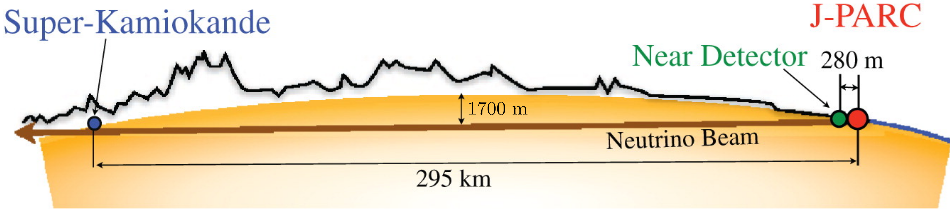
\includegraphics[scale=0.6]{T2K}
 \caption{The path of the neutrino beam produced in the T2K experiment~\cite{ABE2011106}.}
 \label{fig:t2k}
\end{figure}

The INGRID detector lies on the axis of the neutrino beam, but ND280 and SK are 2.5\degree\ off-axis, which sets the peak of the neutrino flux at 600~MeV, the energy at which muon neutrino disappearance is most likely using current oscillation parameter values.

The content of the neutrino beam used in T2K can be switched between muon neutrinos (\numu) and anti-neutrinos (\anumu). The pions of a certain charge produced in the collisions between the protons and the graphite target are focused by electromagnetic horns. Reversing the current passed through the horns causes particles of opposite charge to be focused and pions with the original charge are deflected, hence one can focus positive pions ($\pi^+$) or negative pions ($\pi^-$) depending on the current's direction. The mode in which $\pi^+$s are focused to give a \numu \ beam is the forward horn current (FHC) mode. To focus $\pi^-$s and create a \anumu \ beam the reverse horn current (RHC) mode is needed.

In the next section, details on T2K's ND280 detector and its proposed upgrades for the next phase of data-taking are given. Information on the other T2K detectors and the beamline is given elsewhere~\cite{ABE2011106}.

\section{ND280: Current State}
ND280 gathers data on the neutrino beam to estimate the beam's flux, energy spectrum, and flavour content. This allows comparison with measurements at the far detector, leading to calculations of neutrino oscillation parameters by observing how the flavour content of the beam has changed as a function of energy. 

As well as monitoring the beam characteristics, ND280 also takes data for neutrino cross-section measurements, providing the community of neutrino oscillation experiments with data to evaluate their interaction models. 

The detector can be broken down into three sub-detectors: a $\pi^0$ detector (P\O D), a tracker consisting of two fine grain detectors (FGDs) and three time-projection chambers (TPCs), a system of electromagnetic calorimeters (ECals), and a side muon range detector (SMRD). The whole detector is subject to a 0.2~T magnetic field for charge identification and momentum determination. See Fig.~\ref{fig:ND} for a visualisation of the ND280 detector, its sub-detectors, and the $xyz$ axes used to describe detector orientations in the rest of this section.
\begin{figure}
 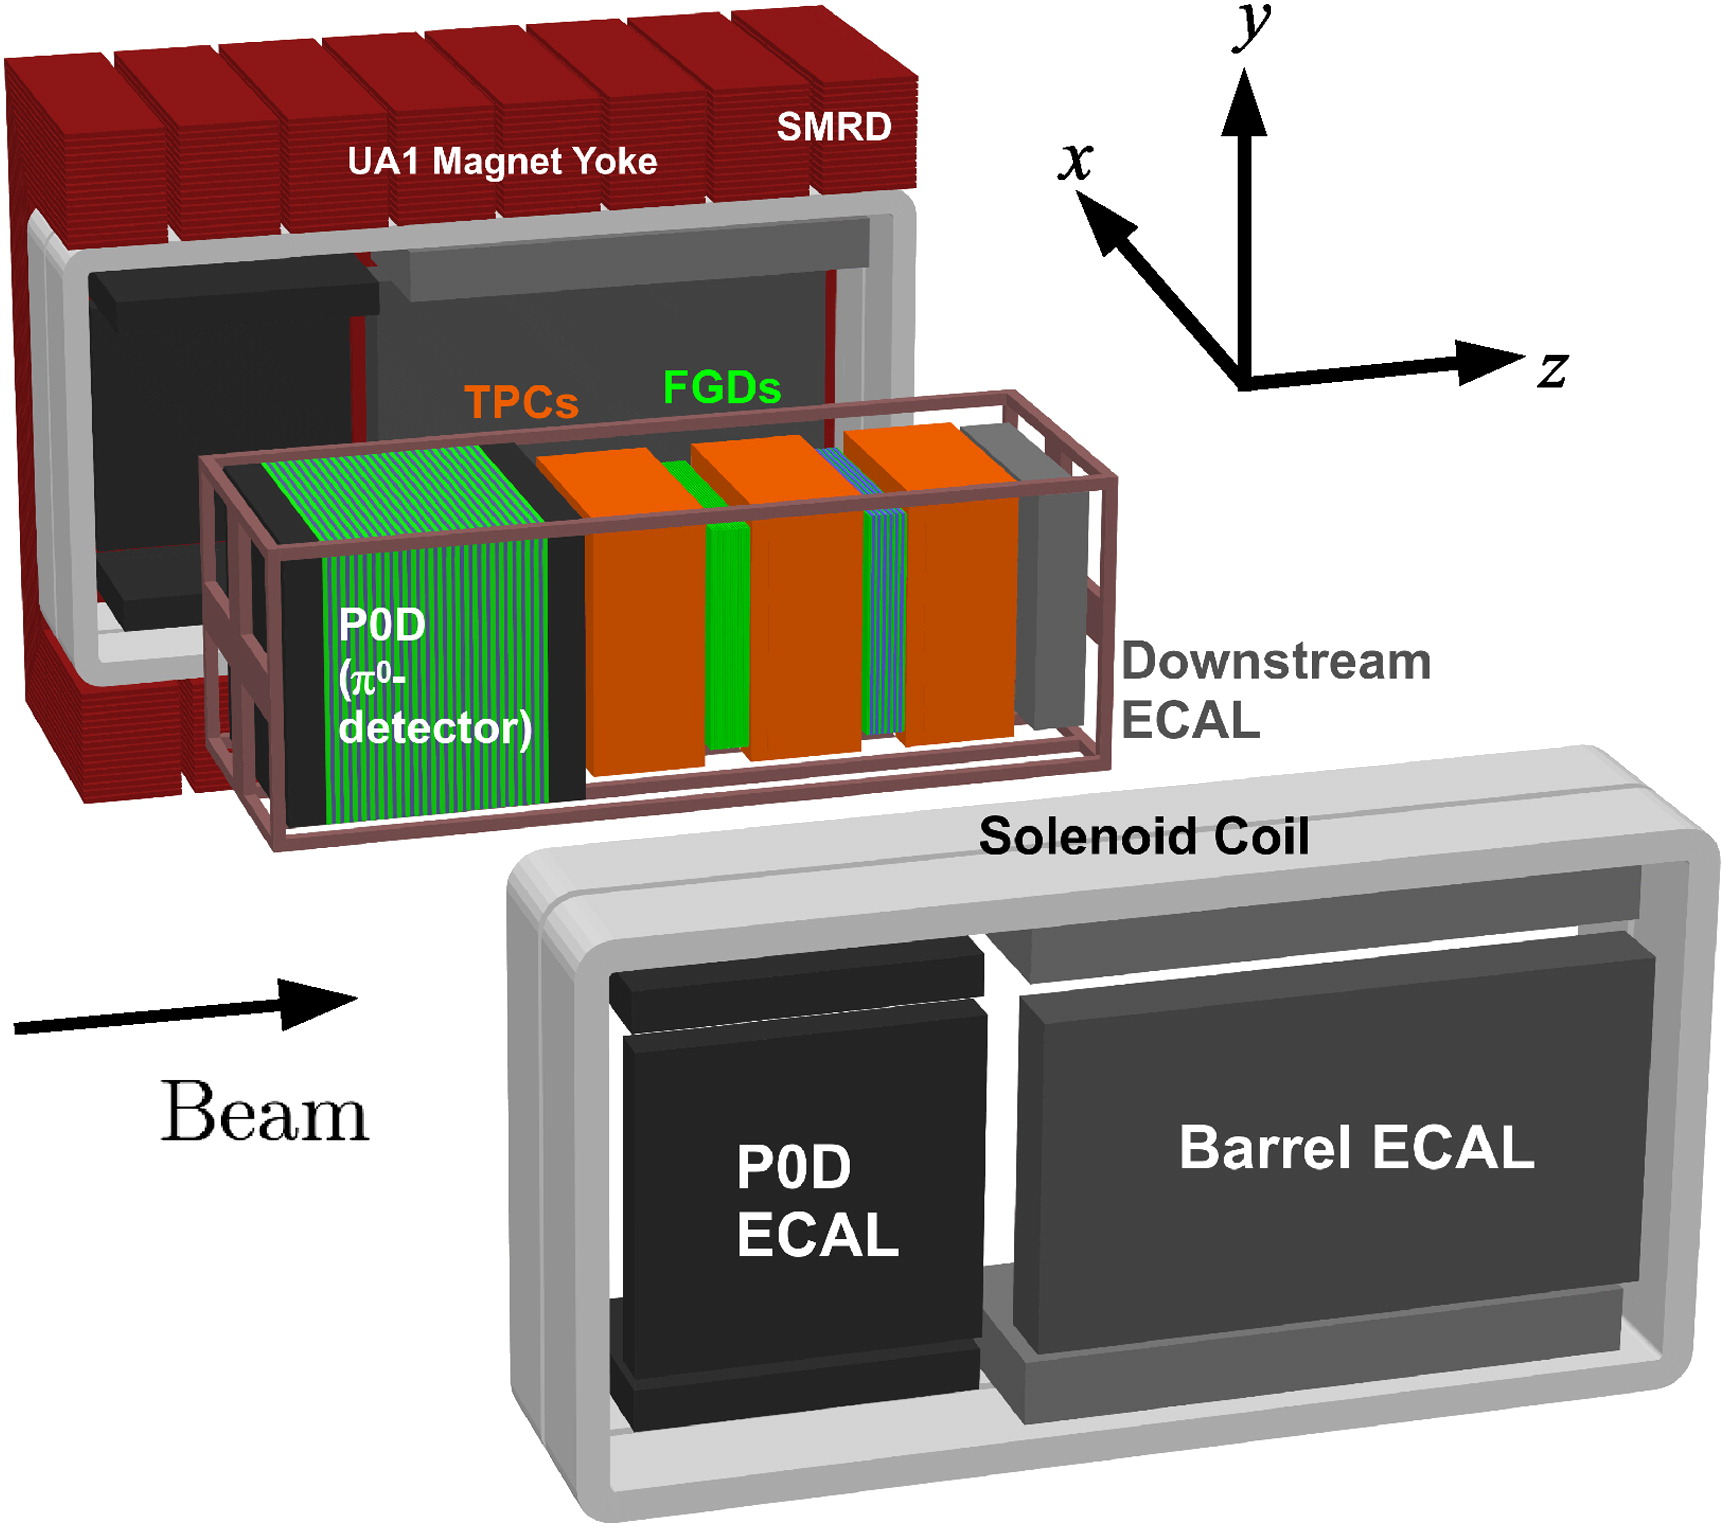
\includegraphics[scale=1]{ND280.png}
 \caption{Expanded view of the ND280 detector, showing the positions of each of the three main sub-systems and sub-detectors. The entire detector is encased in the UA1 magnet with a 0.2~T magnetic field~\cite{ABE2011106}.}
 \label{fig:ND}
\end{figure}

\subsection{\boldmath$\pi^0$ Detector (P\O D)}
T2K's far detector, SK, has difficulty discerning between electrons and the double gamma signal produced in neutral pion ($\pi^0$) decay. To reduce this systematic uncertainty, the P\O D sub-detector of ND280 is used to measure the cross-sections of neutrino interactions, specifically with water, where a $\pi^0$ appears in the final state. Using this cross-section data, the number of $\pi^0$s produced in SK can then be calculated and taken into account. 
%However, in reality these cross-sections are rarely used. The reason for this is the relatively large value of $\theta_{13}$, which means we see significantly more muon neutrinos oscillating to electron neutrinos at SK than $\pi^0$s. The value of $\theta_{13}$ was not known before the P\O D's construction, so it was made as insurance in case the value of the mixing angle turned out to be small.

The central section of the P\O D consists of alternating layers of brass, plastic scintillator, and fillable water bags. The brass acts as a radiator, causing electrons produced by pion decays to shower, whereas the water and plastic layers provide a target for neutrinos to interact with. Plastic scintillator has the useful property of emitting photons when a charged particle passes through it. This is exploited by using wavelength shifting (WLS) fibres to read off the light signal from a passing particle and using the data to reconstruct the particle's trajectory. 

The central target is preceded and followed by electromagnetic calorimeters comprised of alternating sheets of lead and scintillator. These ECals are used for rejecting particles entering the P\O D that originated from outside the detector and also to contain and measure electromagnetic showers. 

Cross-section values with respect to the water target can be deduced by taking measurements when the target bags in the central section are filled with water and comparing them with when they are filled with air~\cite{ABE2011106, Assylbekov:2011sh}.

\subsection{Fine Grain Detectors (FGDs)}
The FGDs provide 2.2 tonnes of mass with which incoming neutrinos can interact and precision tracking to map out the interaction vertices. They consist of bars of plastic scintillator oriented perpendicular to the neutrino beam and stacked side-to-side to form sheets. Two sheets are placed one after the other to form a module, with the bars of one layer being arranged vertically (along the $y$-axis) and the other layer horizontally (along the $x$-axis). The bars are read-off by WLS fibres, so the position of a charged particle incident on a module can be determined in two dimensions. Placing several modules in sequence then gives the trajectory of a particle through the detector

There are two FGDs in ND280. The downstream FGD also contains layers of water in between the scintillator layers. Comparing interaction rates between the two FGDs allows calculation of the cross-sections of neutrino interactions with carbon and water~\cite{ABE2011106, Amaudruz:2012agx}.

\subsection{Time Projection Chambers (TPCs)}
There are three TPCs in ND280, sandwiching the two FGDs. The bulk of each TPC consists of 3000 litres of an argon-based gas. When charged particles pass through this gas, they ionise the gas molecules. The ionisation electrons drift away from a cathode and towards a readout plane. The location and arrival time of the electrons on this plane can be used to construct a 3D image of the particle's trajectory.

TPCs are ideal for identifying the number and trajectory of charged particles in the detector, although their relatively small mass makes it unlikely for a neutrino to interact with them, hence the need for FGDs. The information provided by TPCs allows selection of low-contamination interaction samples, as well as momentum measurements from curved tracks caused by the magnetic field present in the detector. Combining a particle's momentum along with the ionisation of the particle's track, one can identify the type of particle that made the track. Hence, when combined with the FGD data, the TPCs can be used to help identify neutrino interactions in ND280 and to determine the electron neutrino contamination in the muon neutrino beam~\cite{ABE2011106, Abgrall:2010hi}.

\subsection{Electronic Calorimeter (ECal)}
As well as the ECals either end of the P\O D, there are also ECals surrounding the entire detector. A ``barrel'' ECal encompasses the tracker around the $z$-axis, another ECal is situated downstream of the tracker, and a third encircles the P\O D about the $z$-axis. 

The main uses of the ECals are to complement the inner detectors by measuring the energies of photons missed by the inner detectors, reject particles from interactions outside the detector, and help with particle identification.

Alternating layers of scintillator and lead absorber make up each ECal. The scintillator layers consist of several bars of plastic scintillator. These bars are oriented perpendicular to the scintillator bars of the adjacent layers, similar to the FGDs~\cite{ABE2011106}.

\subsection{ND280 Software}
The ND280 software is used for offline analysis of data collected by ND280, as well as Monte Carlo (MC) data generation and analysis. The basic framework of the code was built in 2004, with the underlying structure and data storage relying on ROOT~\cite{Brun1997}, simulation libraries from Geant4~\cite{Agostinelli2003}, a package management system provided by CMT (Configuration Management Tool) \cite{Arnault:2000vu} and the version control system used to store each version of the code is CVS (Concurrent Version Systems) \cite{Berliner2001}.

A decision was made early-on in the software's lifetime to split the structure of the software into different packages, resulting in about 60 software packages in total~\cite{ABE2011106}. This offers easy access to specific areas of code and makes editing the software simpler for developers. 

The flow-path of the different data types through the package structure is shown in Fig.~\ref{fig:struct}, 
\begin{figure}
 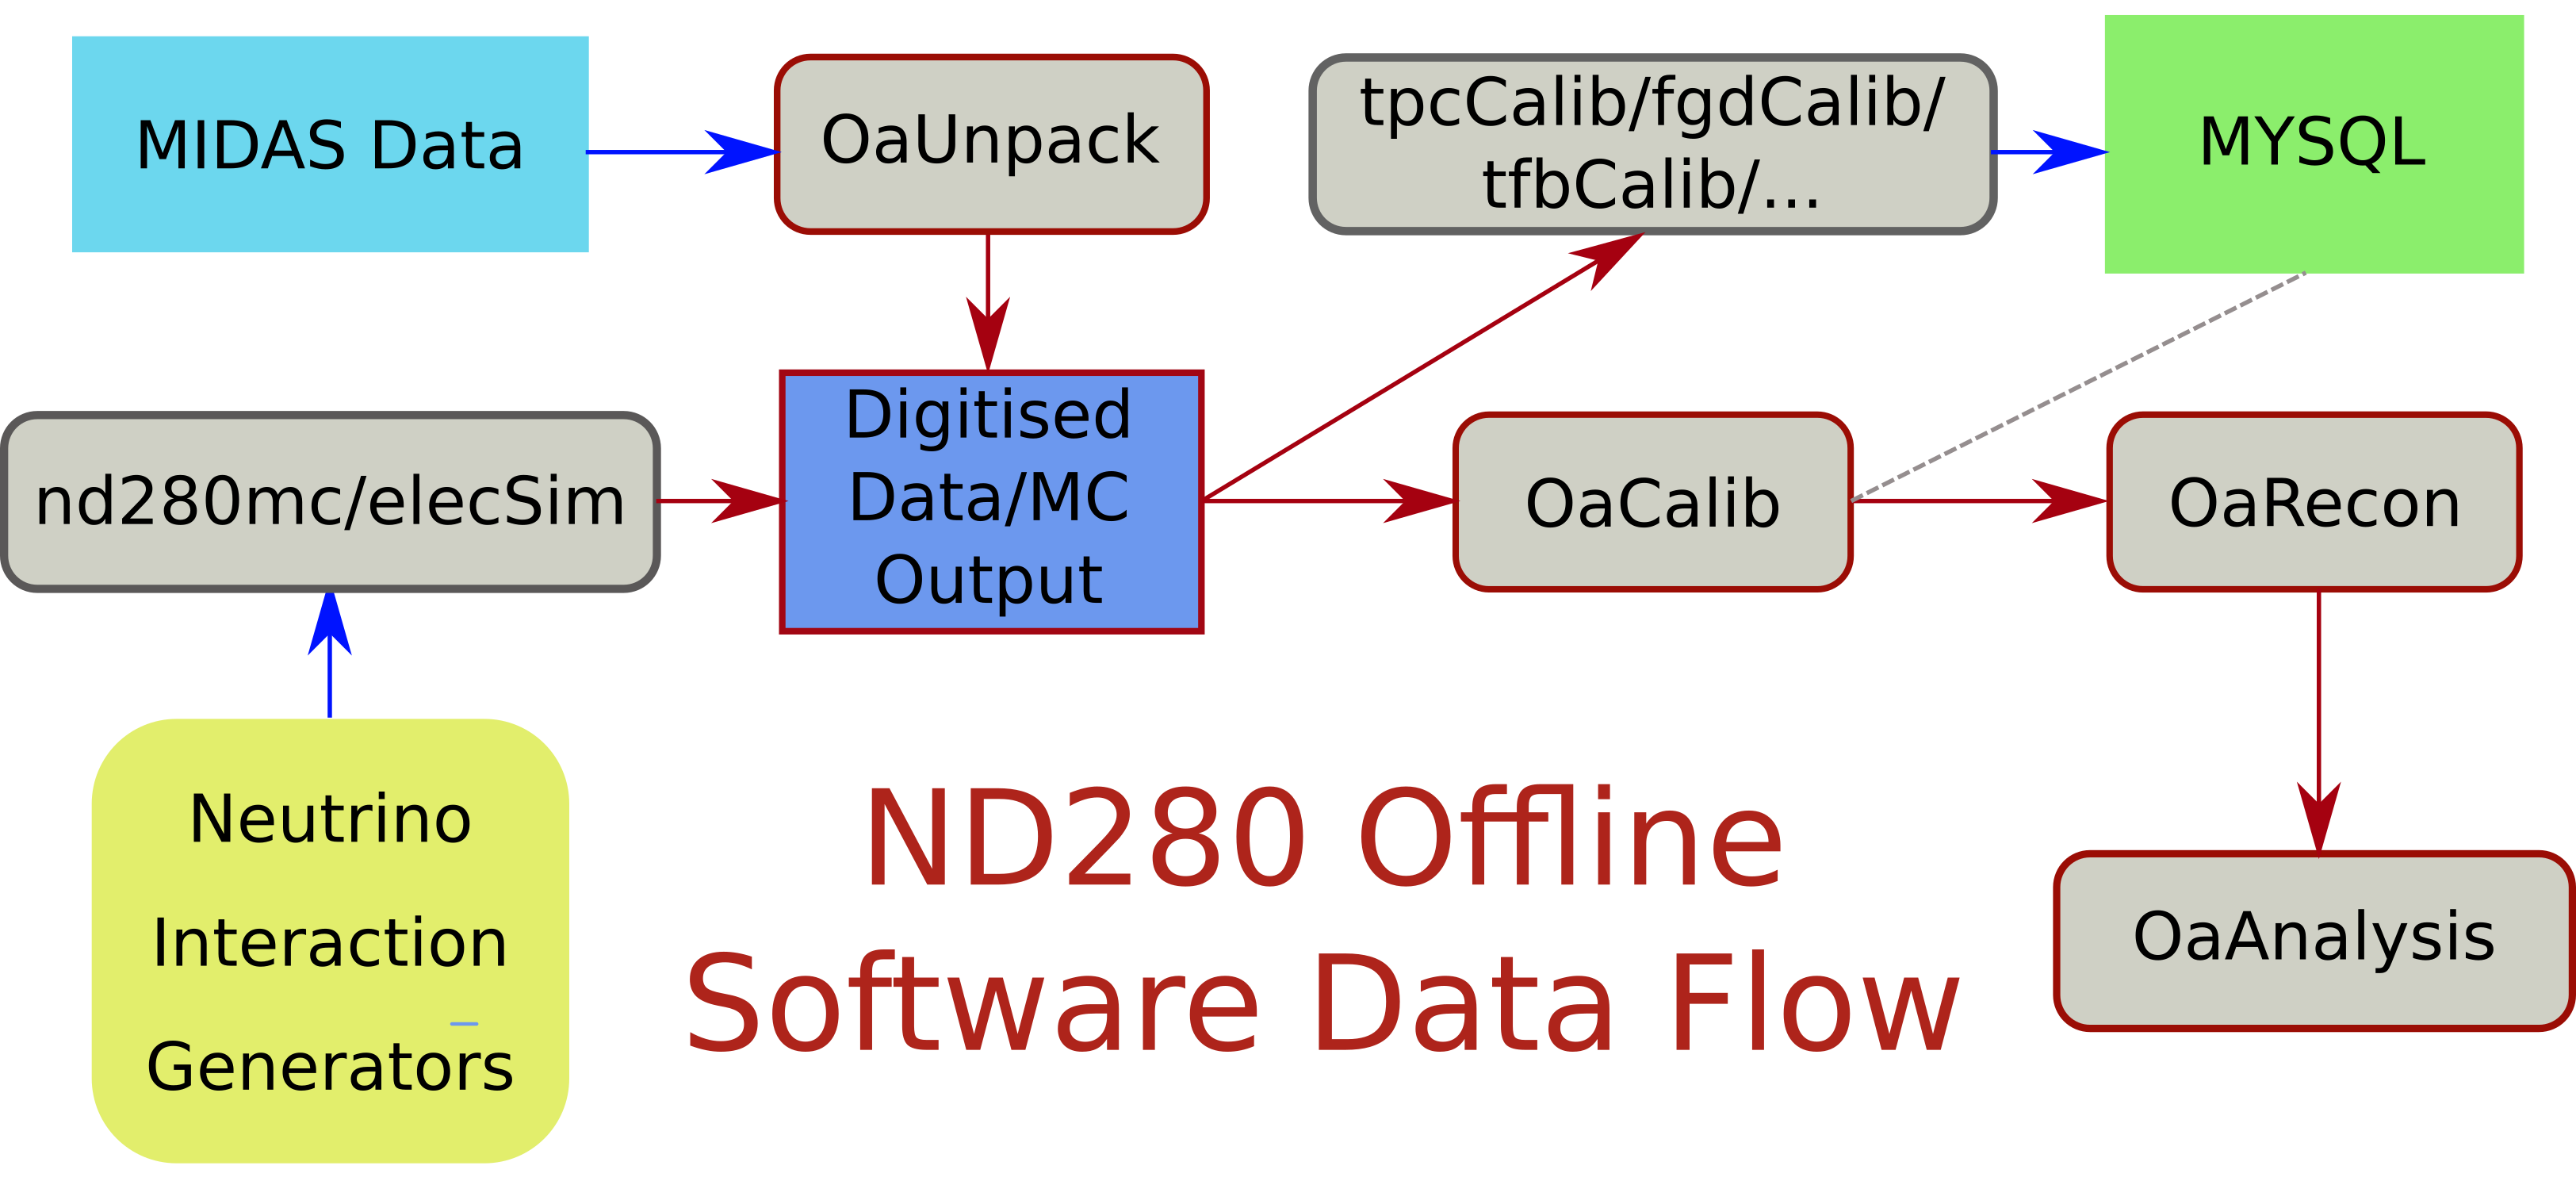
\includegraphics[scale=0.5]{dataflow.png}
 \caption{The flow of data through the package structure of the ND280 software. The flow is simplified and only shows the most relevant packages. Boxes with red coloured borders represent packages that process oaEvent data.}
 \label{fig:struct}
\end{figure}
but only the most relevant packages are shown.

The package oaEvent (the ``oa'' prefix stands for ``off-axis'') is important as it defines the format of the data passed through the software between the steps where raw MIDAS data (MIDAS is the format of data from the ND280 detector \cite{Ritt2001}) is passed to the software and the final step where oaAnalysis reduces the data to a user-friendly format. The oaUnpack and oaRawEvent packages handle the conversion of MIDAS data to oaEvent data. oaCalib then applies calibration constants to the data, whilst oaCalib's sub-packages use the data to produce calibration constants to store in MYSQL, which are used by oaCalib. The data is then passed on to oaRecon, which uses the data to reconstruct the particle events that occurred in the detector, the results of which are analysed by oaAnalysis.

The exact same processes are applied to MC generator data, except that the data does not start in MIDAS format. The MC data is produced by passing information from the neutrino flux packages to the neutrino interaction generators NEUT~\cite{Hayato:2009zz} and GENIE~\cite{Andreopoulos2010}. These generators produce realistic distributions of child particles from neutrino interactions. The simulation is then taken over by nd280mc, which uses Geant4 to propagate the child particles and simulate the energy deposits left in the detector. elecSim then converts these energy deposits to simulated electrical readouts, as would be seen in the real detector and recorded in MIDAS format, except here it is written as oaEvent data.
 
\section{Hardware Upgrades}
Resulting from T2K's success in measuring oscillation parameters with improved precision, the experiment is set for a series of upgrades to further increase the measurement precision. In tandem with these improvements, ND280 must also be revamped to reduce systematic uncertainties in the neutrino appearance predictions and cross-section measurements. Here, we will go through the proposed upgrades that are planned for construction over 2019--2020 to be installed in Japan by 2020~\cite{Blondel:2299599}.

\subsection{Scintillator Detector and Horizontal TPCs}
The proposed upgraded ND280 is shown in Fig.~\ref{fig:up}.
\begin{figure}
 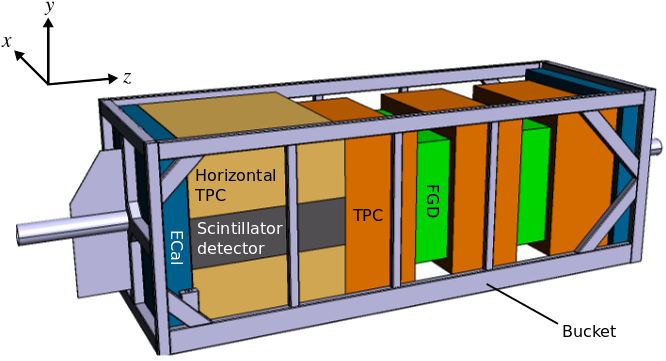
\includegraphics[scale=0.5]{upgrade2.png}
 \caption{The proposed upgrade of ND280. The new additions are the horizontal TPCs and the scintillator detector, which replace the P\O D. The ``bucket'' is a framework that supports the detectors. Not shown are the barrel ECals that will surround the detectors, similar to the original design. The neutrino beam propagates in the $z$ direction~\cite{Blondel:2299599}.}
 \label{fig:up}
\end{figure}
The downstream end of the detector will remain unchanged, with three TPCs separated by two FGDs followed by an ECal. At the upstream end, however, the central P\O D module (not the ECal endcaps) will be replaced by a scintillator detector sandwiched between two horizontal TPCs. The reason for the P\O D's removal is the large value of $\theta_{13}$, making its measurements to estimate the double gamma backgrounds at SK less necessary than previously thought, as the background is significantly smaller than the observed signal. 

The scintillator detector will act as a target material, with the TPCs distributed around it giving nearly 4$\pi$ solid angle coverage. This will address an issue with the old ND280 design: the tracking efficiency is biased towards low scattering angles. This is because, after a neutrino has interacted in an FGD, the resulting lepton is only seen clearly in the downstream TPC if the scattering angle is less than about 40\degree\ with respect to the beam direction. The TPC gives important information on the interaction, so most interaction samples exclude leptons with high scattering angles. This creates problems when comparing data with SK, which has a flat efficiency with respect to scattering angle.

The new scintillator detector will have a first-of-its-kind ``Super-FGD'' design that incorporates scintillator cubes rather than bars, which can be read out from three orthogonal directions by WLS fibres. The cubes' side length will be between 1--2~cm, with the larger lengths sacrificing granularity for a smaller number of cubes and readouts. The size of the cubes is comparable to the height and width of the scintillator bars used in the current design, but the bars only readout in two directions. The extra information provided by the cubes helps to reconstruct the paths of multiple particles. This means it will be easier to discern electrons produced from neutrino interactions from electron-positron pairs produced by gamma particles. It will also give larger data samples of multi-nucleon final state interactions, which are one of the main contributors to systematic uncertainties in analyses. Fig.~\ref{fig:sfgd}
\afterpage{
 \begin{figure}
  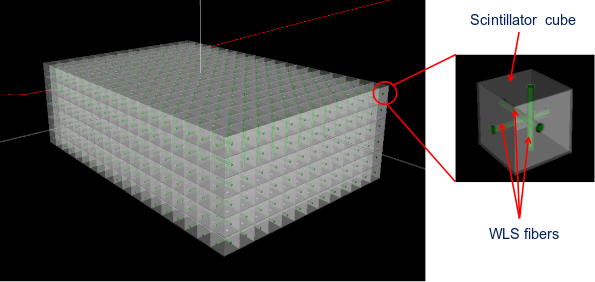
\includegraphics[scale=0.75]{SFGD.png}
  \caption{A rendering of the Super-FGD to be used in the upgraded ND280. The detector comprises many small plastic scintillator cubes that are read off in three orthogonal directions by wavelength shifting fibres. There are fewer cubes depicted here than there will be in the actual detector, to make the diagram clearer~\cite{Blondel:2299599}.}
  \label{fig:sfgd}
 \end{figure}
}
shows an illustration of the Super-FGD design.

Prototypes of the horizontal TPC and the Super-FGD will be used in test-beams at CERN, the latter of which is being tested at the time of this report being submitted. Details of the Super-FGD's beam test will be given in Sec.\ \ref{sec:sfgd}.

\subsection{Time of Flight Detectors}
Not shown in the diagram of the ND280 upgrade (Fig.~\ref{fig:up}) are the new time-of-flight (TOF) detectors that are to be installed. These will be placed around the volume containing the scintillator detector and the horizontal TPCs. The TOF detectors will help identify whether a particle originated from inside or outside the detector and will also aid with particle identification. The design of the TOF detectors is as yet undecided. There are two possible candidates, one based on wavelength shifting fibres and the other based on plastic scintillator bars. A prototype of the latter design is being constructed in 2018 and will be tested later in 2018~\cite{Blondel:2299599}. 

\section{Super-FGD Beam Test}
\label{sec:sfgd}
The beam test for the Super-FGD prototype is scheduled for June 27th -- July 11th 2018, taking place at CERN using the T9 beam line.

The main goals of the beam test are:
\begin{itemize}
 \item Illuminate the detector with roughly 5~GeV muons to ascertain the detector's properties such as time resolution, position resolution, pulse height uniformity, alignment and more. This will also provide an opportunity to calibrate the detector.
 \item Fire gamma particles produced by pion decays at the detector to study the particle identification (PID) between electrons and gamma rays in the device and the two-track separation of electron-positron pairs.
 \item Use an uncollimated beam of hadrons and muons and measure energy loss of particles and study the effects of particles stopping in the detector.
 \item Collect samples of low energy protons from elastic scattering events with pions ($\pi^+ p \rightarrow \pi^+ p$).
 \item Observe high energy pion interactions that produce many particles to test multi-track separation.
\end{itemize}

The results of the beam test will be known after July 11th 2018. The prototype's design, the set-up of the beam test, and the method of photosensor calibration are reported here. Some preliminary data taken on the beam line is also shown.

\subsection{The Super-FGD Prototype}
The prototype scintillator detector measures $24\times48\times8$ cm$^3$ (the actual Super-FGD will be over 200 times larger) and comprises 9216 extruded cubes of polystyrene mixed with p-terphenyl plastic scintillator, each 1~cm long. There are a total of 1728 WLS fibres threaded through the cubes. On one end of each fibre is a plastic connector, with the other end being left bare. The plastic connector attaches to another connector, which houses a multiple pixel photon counter (MPPC) that transmits a signal to the data acquisition (DAQ) system via an electronic cable (MPPCs will be explained later in Sec.\ \ref{sec:mppc}). Two photographs of the prototype are shown in Fig.~\ref{fig:proto}.
 \begin{figure}
  \centering
  \begin{subfigure}{.5\textwidth}
   \centering
   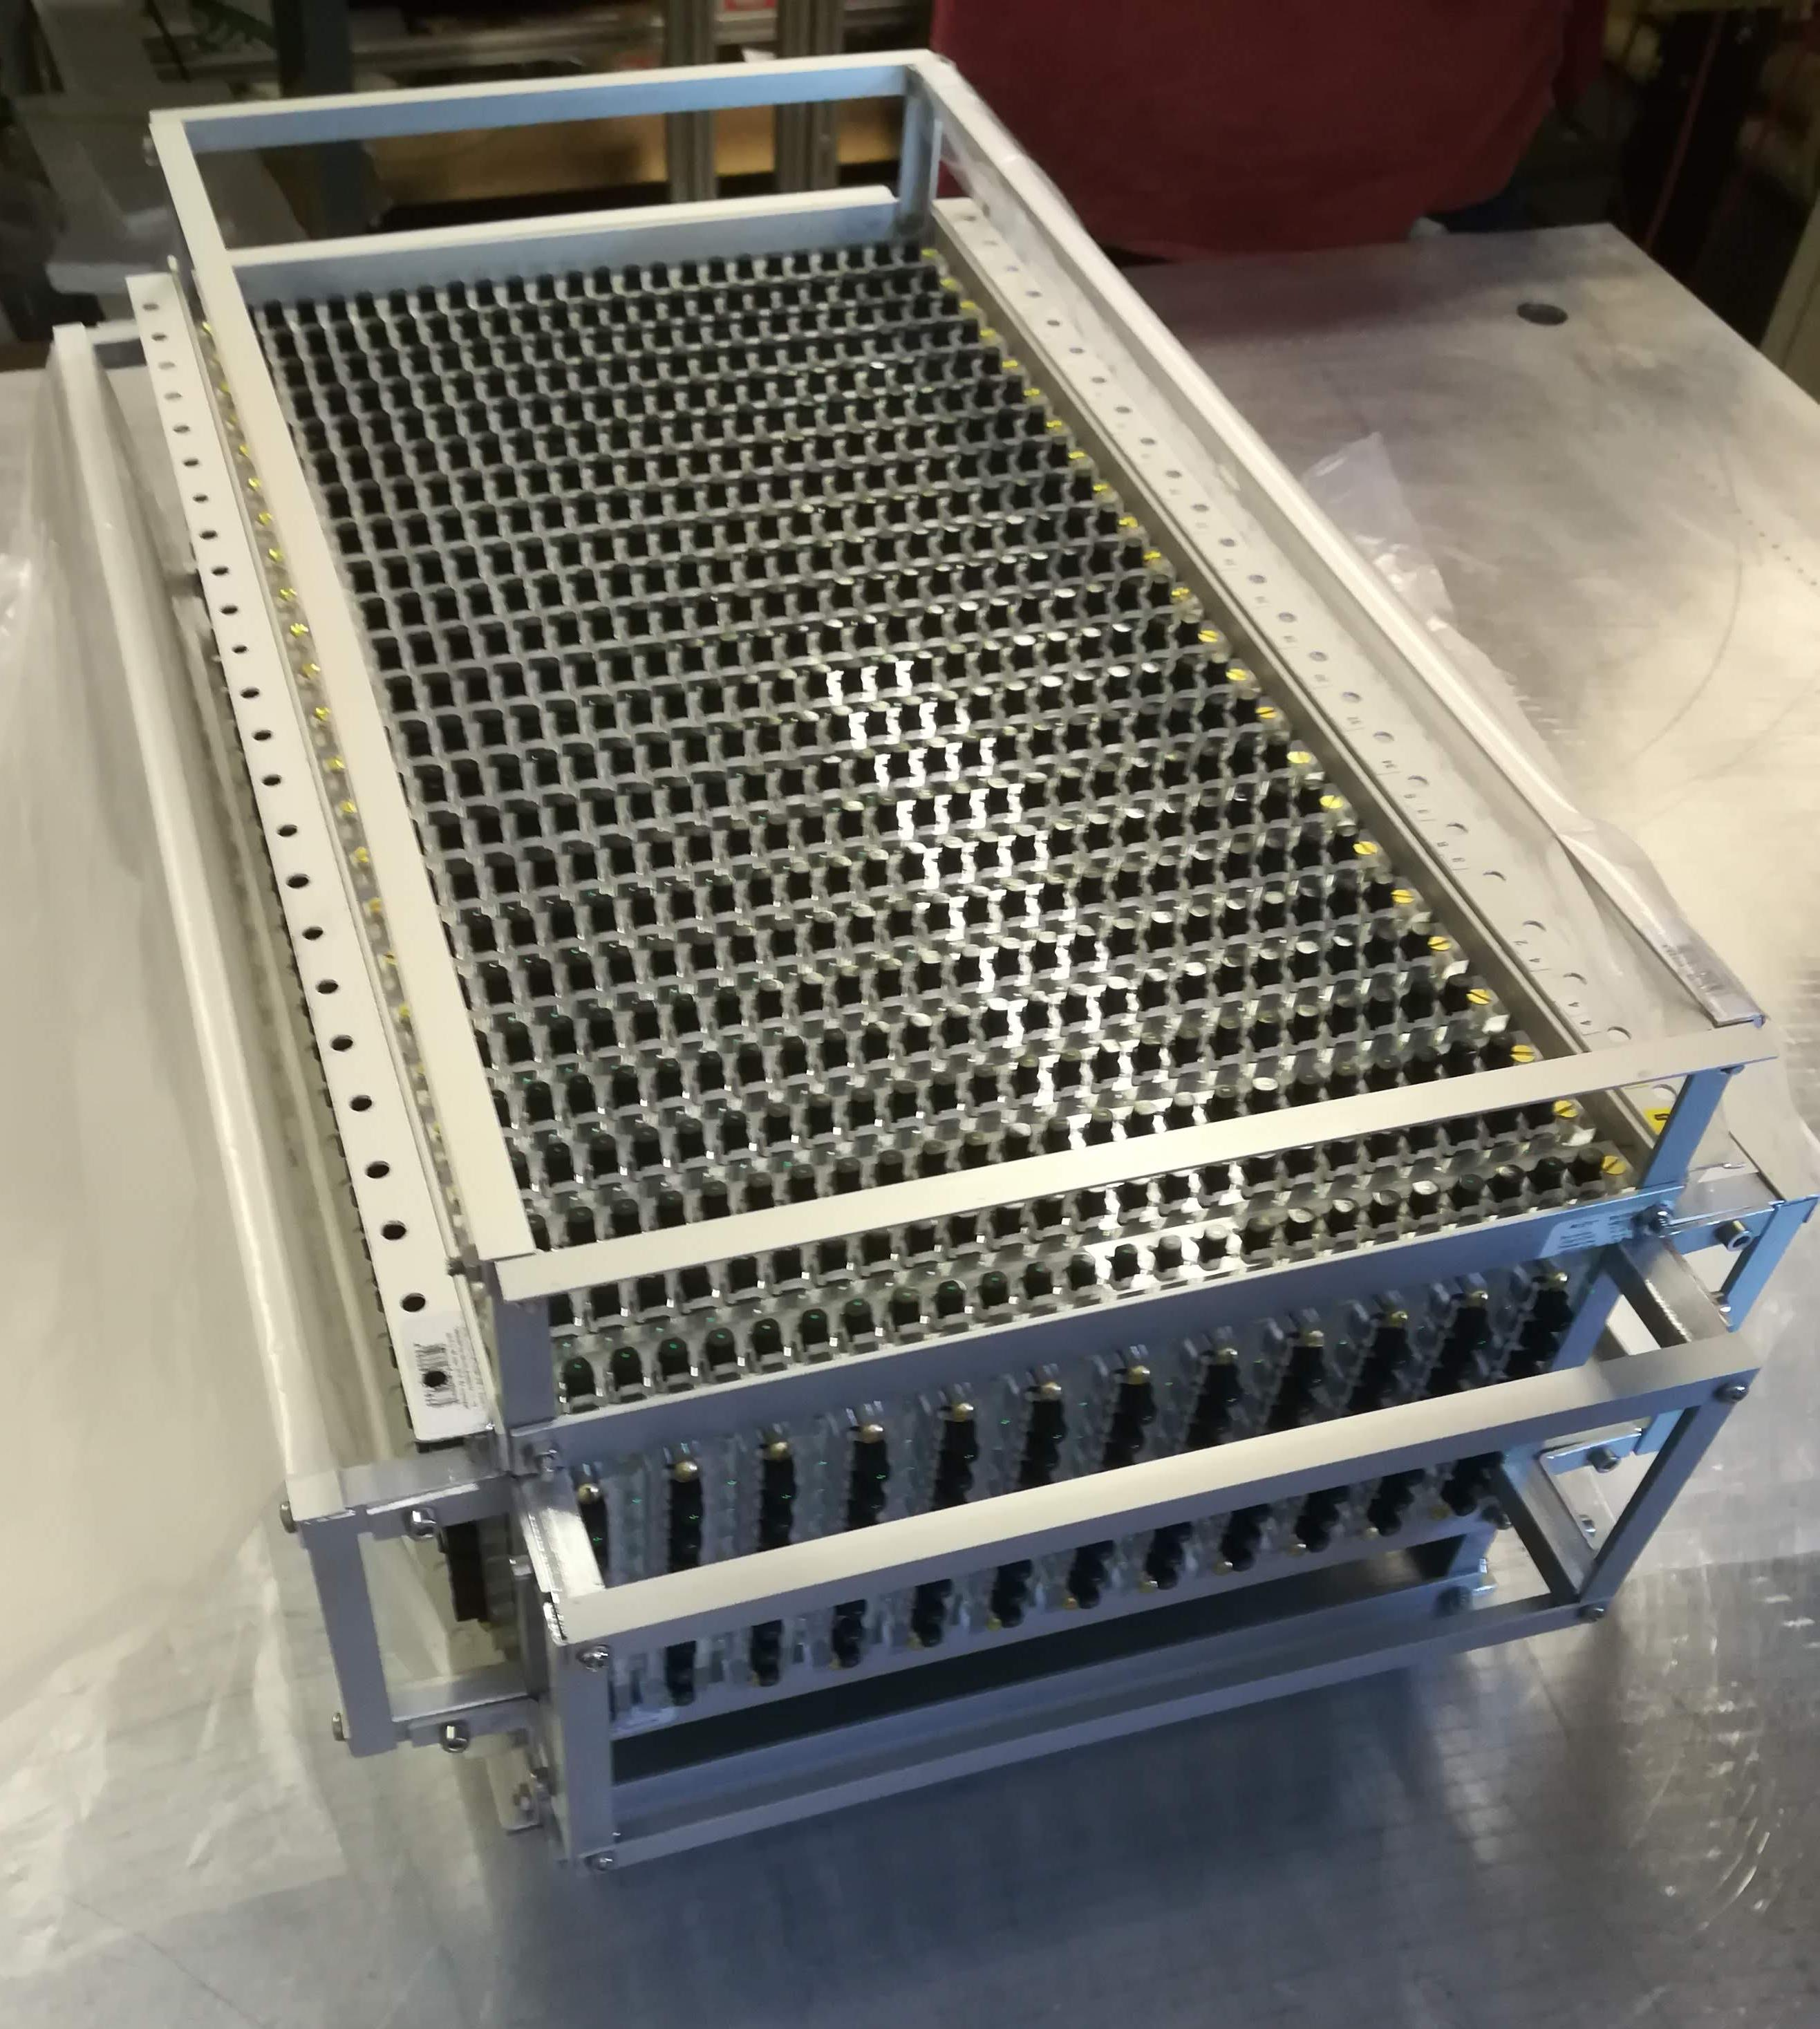
\includegraphics[width=.7\linewidth]{proto}
   \caption{•}
   \label{fig:protoa}
  \end{subfigure}%
  \begin{subfigure}{.5\textwidth}
   \centering
   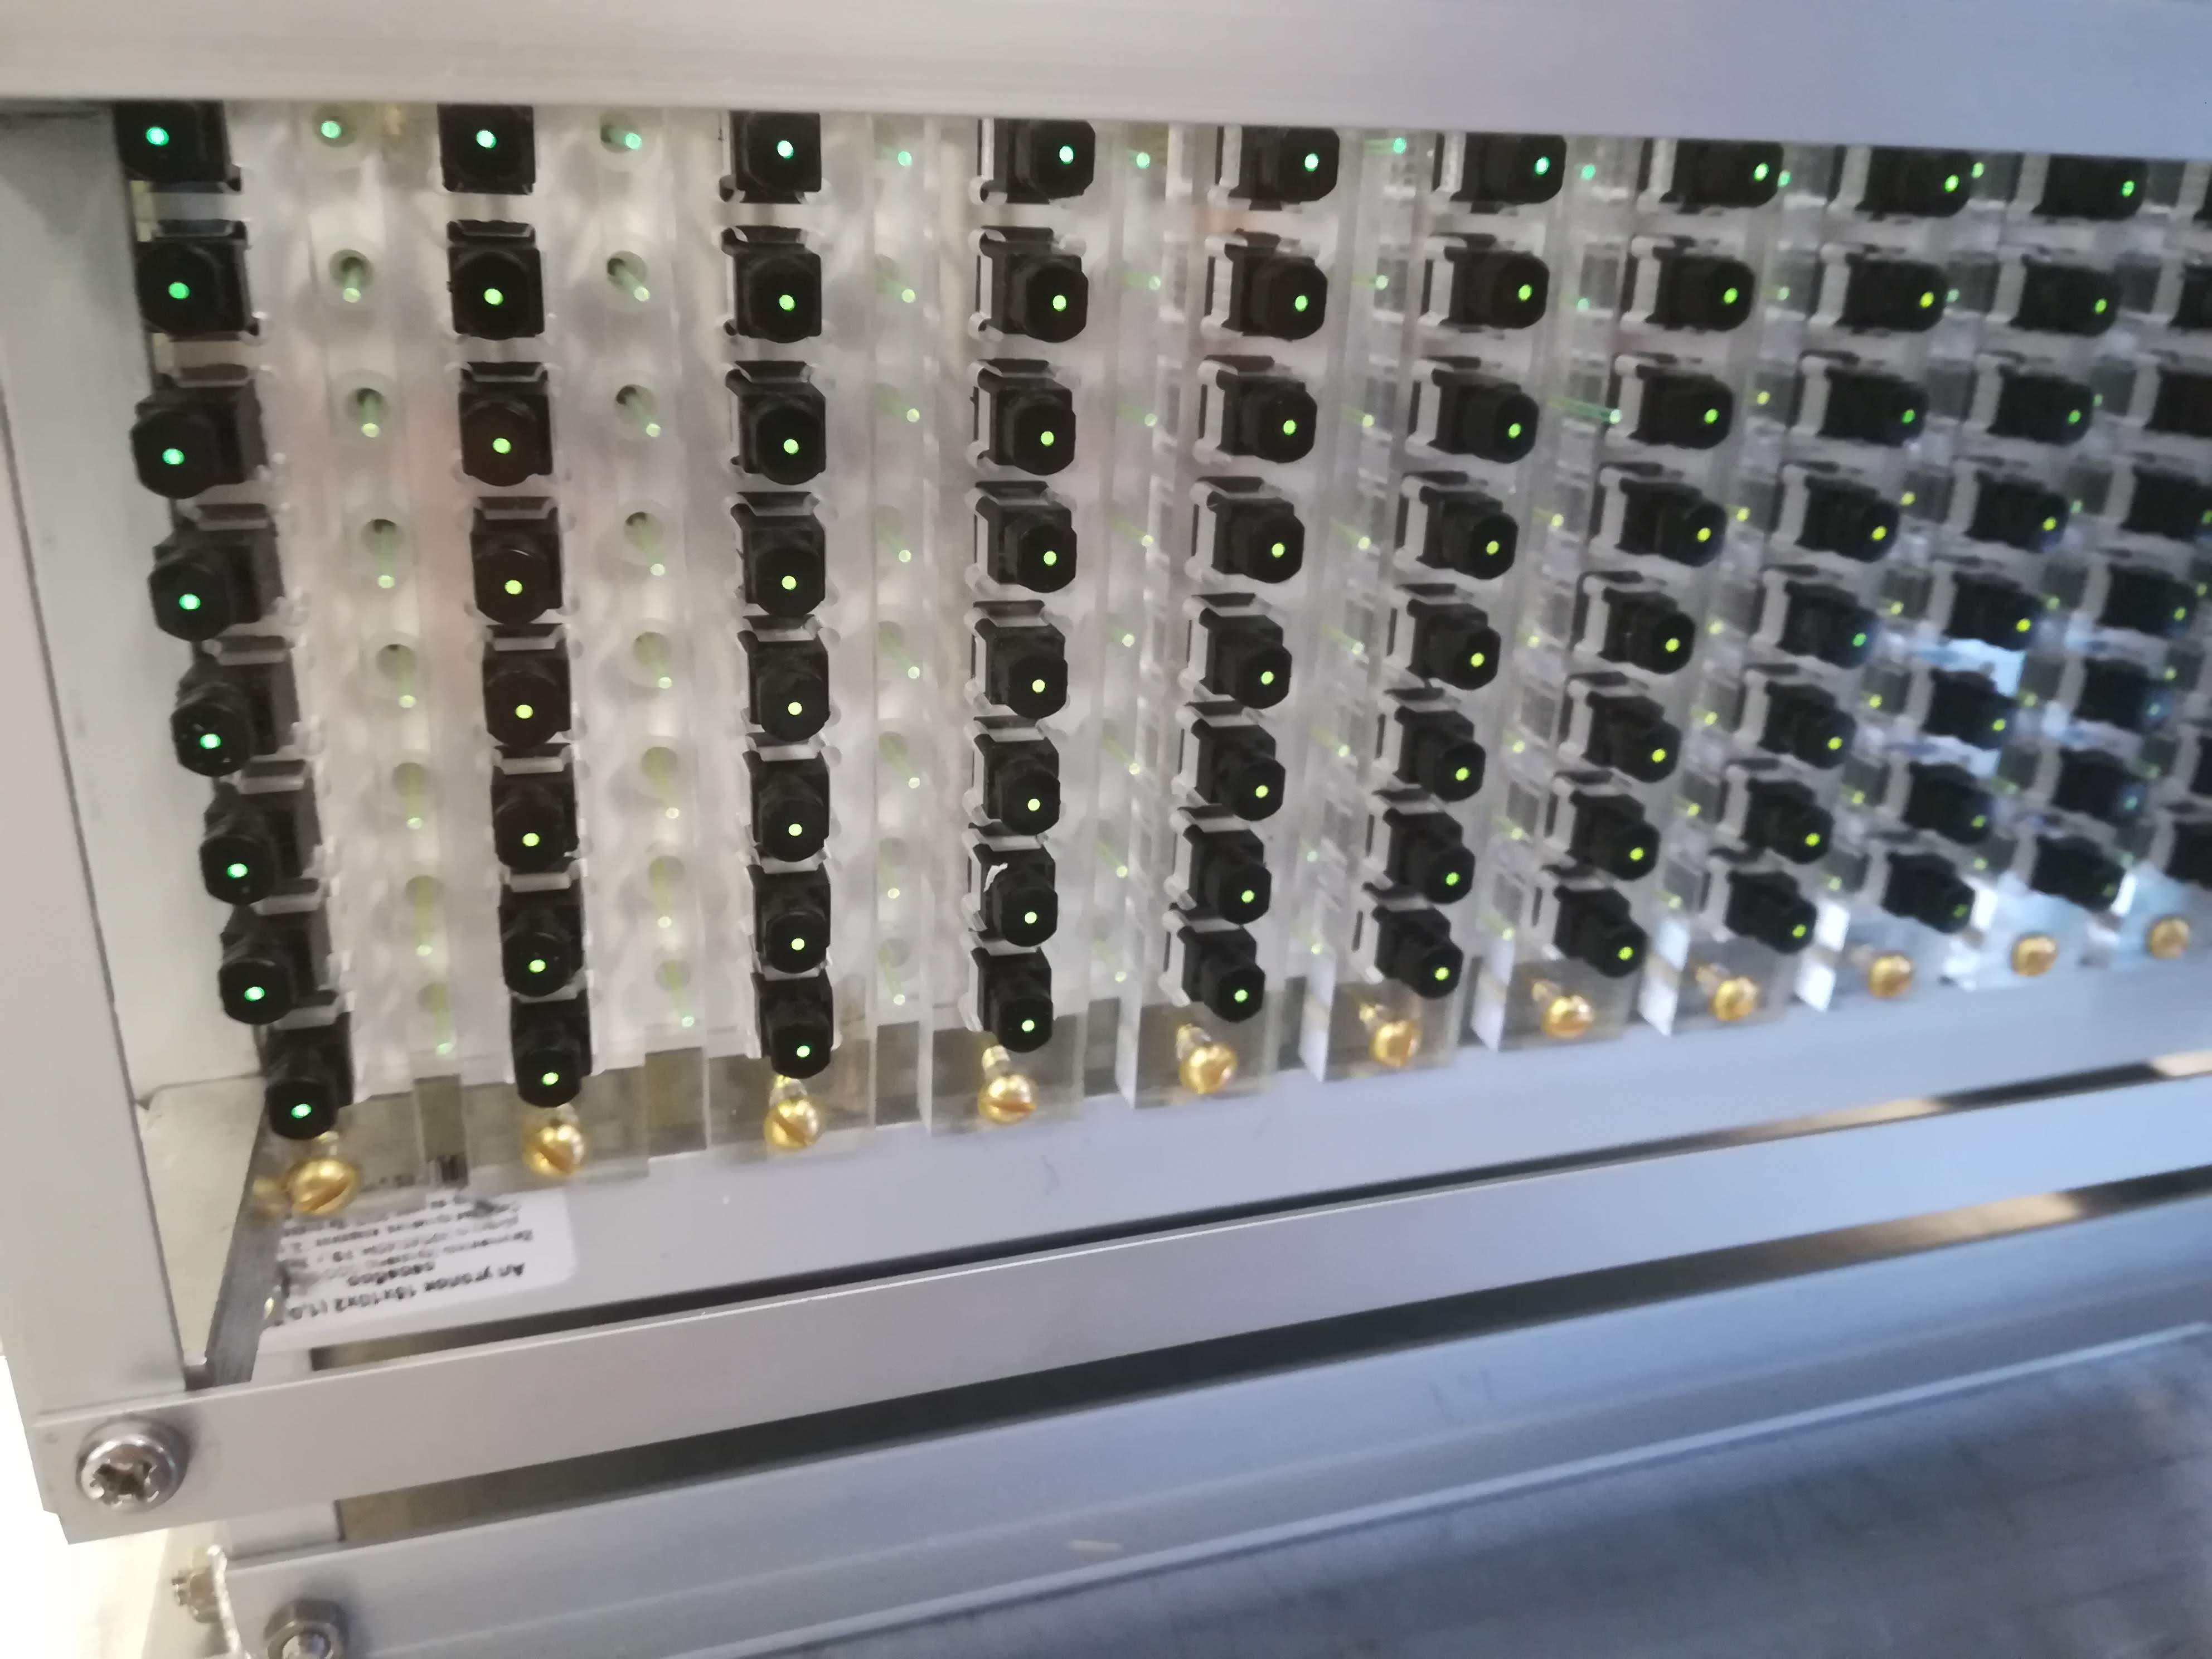
\includegraphics[width=.8\linewidth]{side}
   \caption{•}
   \label{fig:protob}
  \end{subfigure}
  \caption{Photographs of the Super-FGD prototype after being delivered to CERN. These were taken before the electronics were fitted for the beam test. (a) shows the whole detector, along with the frame it is housed in. (b) is a close-up of one of the detector's sides, giving a clear view of the scintillator cubes and the WLS fibres. The black connectors are where the readout electronics will be attached.}
  \label{fig:proto}
 \end{figure}
Fig.~\ref{fig:protoa} shows the construct as a whole, housed in its frame. The frame is used to attach the detector to a sliding platform and the cables connecting the detector to the readout electronics can be tied to the sides of the frame. Fig.~\ref{fig:protob} displays a close-up of the side of the detector, giving a detailed view of the connectors at the ends of the WLS fibres, which will connect the detector to the DAQ system.

\subsection{The Beam Test Configuration}
The beam test is taking place in the East Area of the Proton Synchrotron at CERN. Test-beam T9 is being used to fire $p, \ e^+, \ e^-, \ \pi^+, \ \pi^-, \ \mu^+$ and $\mu^-$ particles at the Super-FGD prototype with momenta ranging between roughly 0.5--5~GeV (this is the expected momentum range for particles to be produced in the ND280 detector)~\cite{Durieu2001}. 

The prototype is placed inside the MNP17 magnet, which is present for momentum measurements~\cite{Brooks2015}. The magnetic flux density is set to 0.2~T, the same as the UA1 magnet of ND280. All readout electronics, such as the circuit boards that process the signal, need to be placed outside the magnet field, hence long cables (about 1.5~m long) are used to connect the detector to the electronics. 

Fig.~\ref{fig:plat}
\begin{figure}
 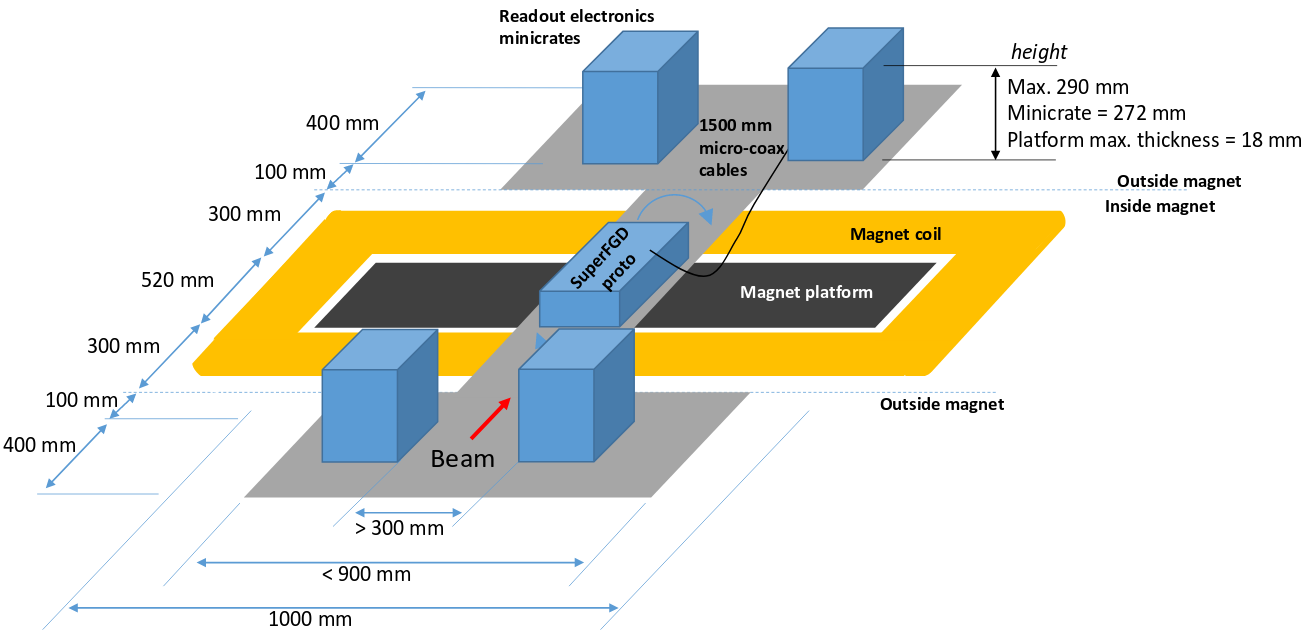
\includegraphics[scale=0.4]{platform2}
 \caption{A plan of the orientation of the prototype detector and its DAQ electronics with respect to the MNP17 magnet. Not shown is the upper platform of the magnet, which sits 290~mm above the lower platform. In order to access the prototype during the beam test, it is placed on a mechanical platform that can slide out of the magnet. The platform also rotates about the horizontal axis parallel to the beam and the vertical axis to allow different orientations of the prototype with respect to the beam~\cite{Cadoux2018}.}
 \label{fig:plat}
\end{figure}
shows how the detector is oriented with respect to the magnet, as well as the readout electronics, which are kept in metal boxes called ``minicrates''. The prototype is kept on a rotating platform so the detector's response to particles incoming at several angles can be tested.

The DAQ system in the minicrates is the same one that will be used for Baby MIND (Baby magnetised iron neutrino detector)~\cite{Antonova2017}. This is used concurrently with another DAQ system using a WaveCatcher digitiser~\cite{CAEN}. The system is connected to several hodoscopes and Cherenkov detectors, which will act as a trigger system and give PID. Baby MIND has its own trigger system, so its results will be compared with those of the WaveCatcher system, as a means of corroboration.

The layout of the detectors used in the trigger system is shown in Fig.~\ref{fig:daq}.
\begin{figure}
 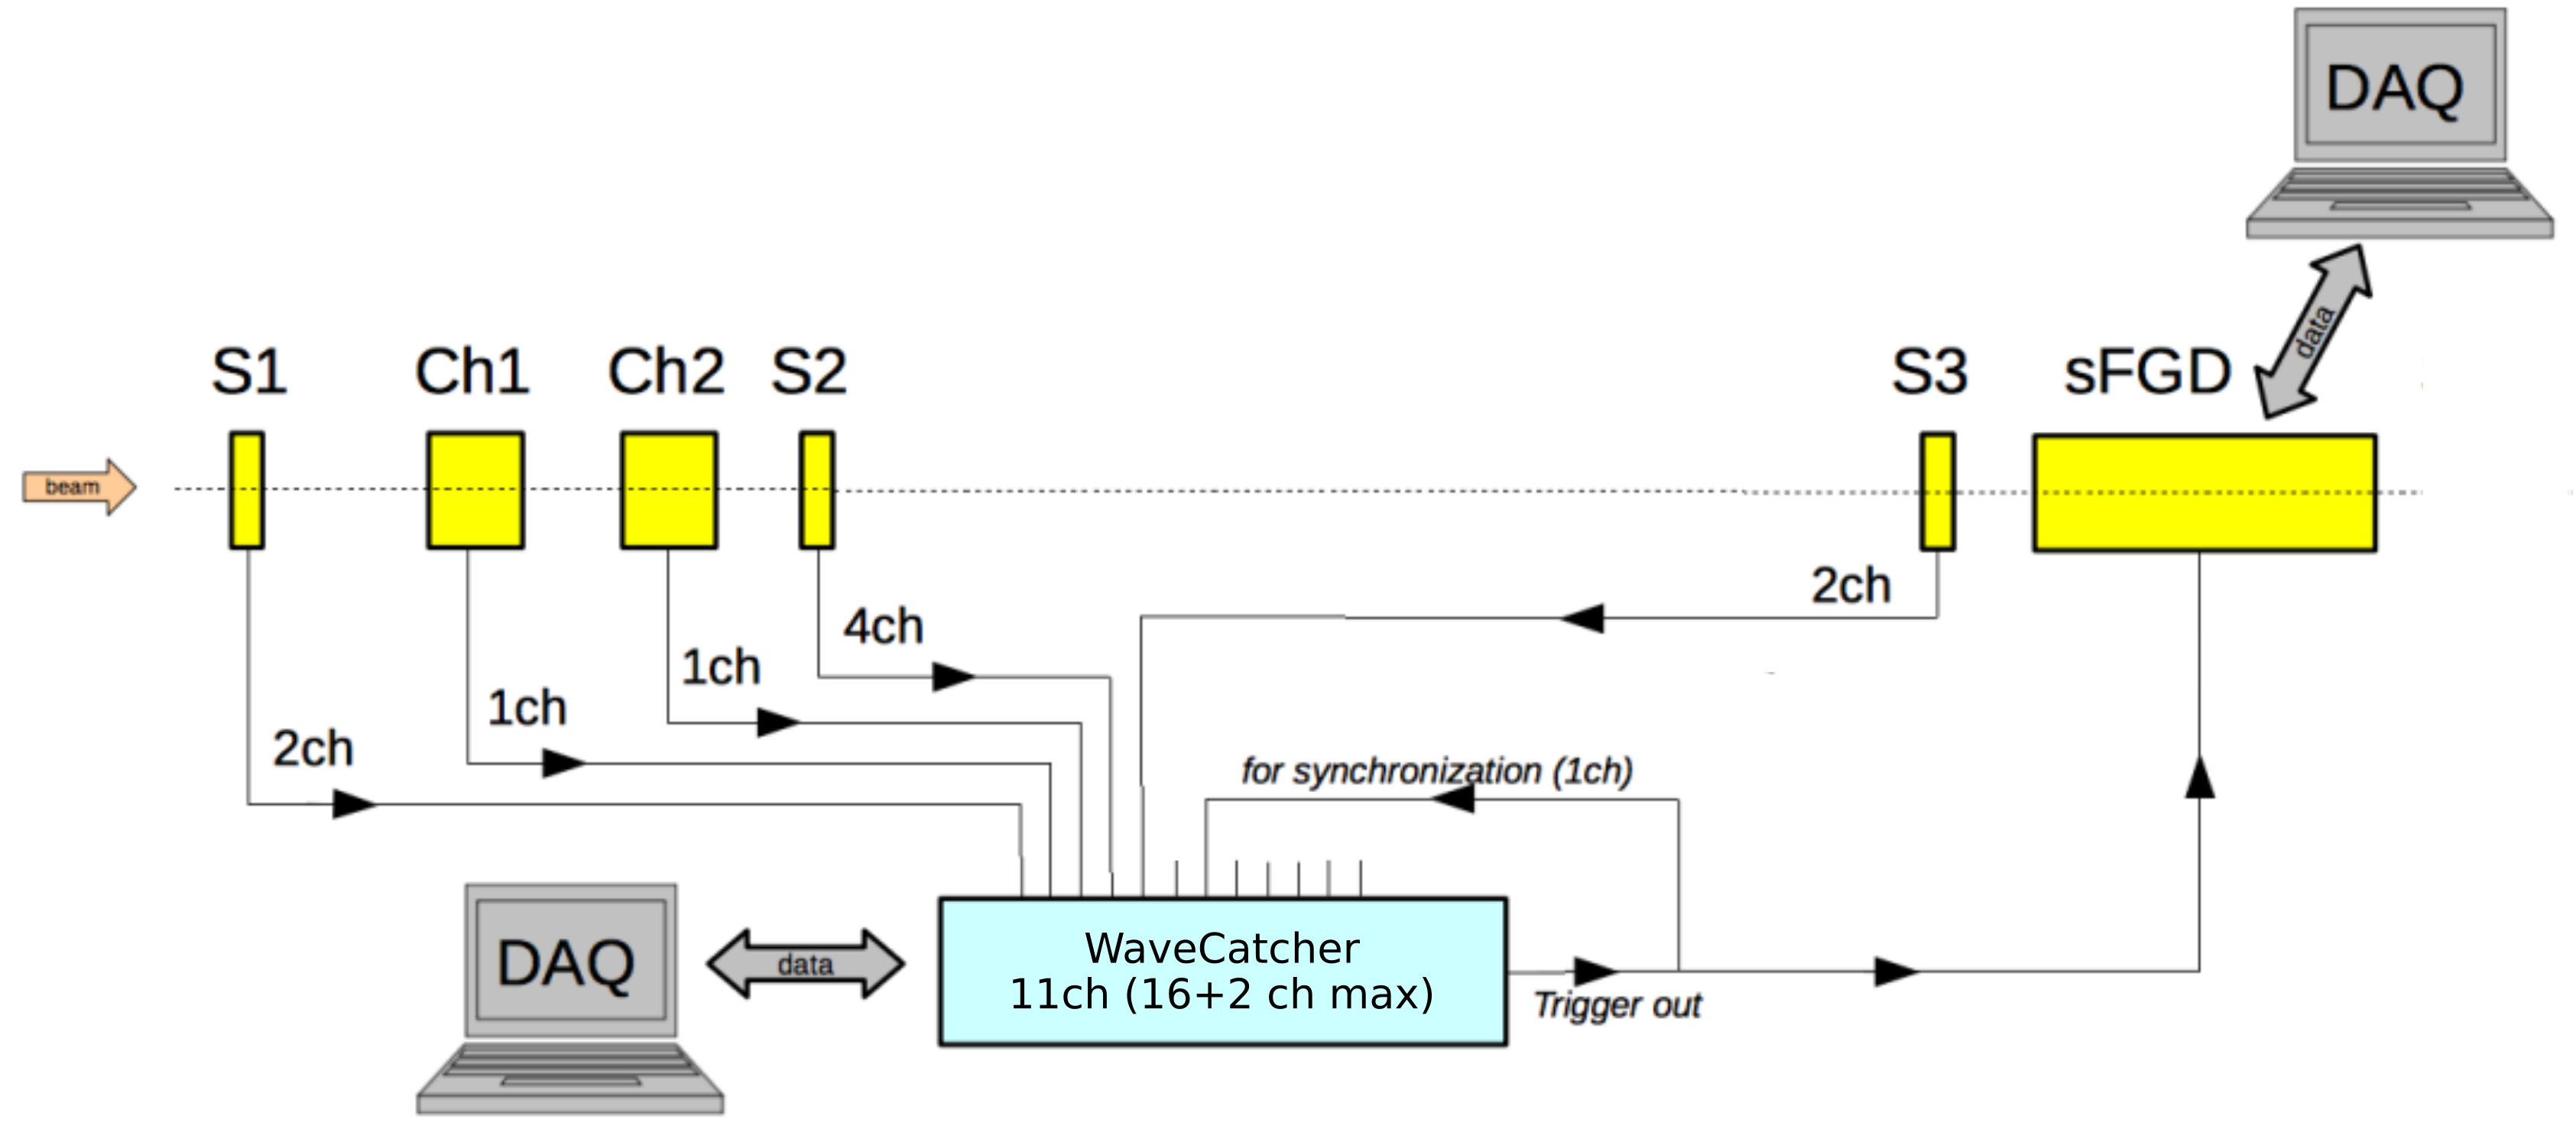
\includegraphics[trim={1px 2px 1px 1px}, clip, scale=0.55]{daq2}
 \caption{A schematic of the layout and DAQ for the beam test. The yellow boxes labelled S are beam scintillator counters and the ones labelled Ch are Cherenkov detectors. These are used in the trigger system for the Super-FGD prototype, labelled sFGD in the diagram. PID can be performed with the detectors in the triggering system by using time-of-flight and Cherenkov signals. There are two independent DAQ systems, one based on the WaveCatcher and the other Baby MIND, which is self-triggering. Also shown are the number of channels (ch) from each trigger component~\cite{Korzenev2018}.}
 \label{fig:daq}
\end{figure}
There are three hodoscopes in total, along with two Cherenkov detectors. By monitoring these detectors the trigger can be activated when a signal is produced in each one within a certain time window. Time of flight information can also be used to distinguish protons from lighter particles. The Cherenkov detectors help with PID by distinguishing electrons from muons and pions. In the 0.5--5 GeV momentum range only electrons produce Cherenkov light in these detectors, making it easy to identify them.
%\subsection{Assembling the Prototype}

\subsection{MPPC Calibration}
\label{sec:mppc}
MPPCs are silicon photomultipliers with a negative bias voltage just above the breakdown voltage of the silicon. An array of Geiger Mode Avalanche Photo-Diode pixels is present on each sensor. When a photon interacts with one of the pixels, a photoelectron is produced. The photoelectron is then accelerated by the bias voltage, creating electron-hole pairs in the silicon as it travels. This results in the initial charge created by the photon increasing significantly, like a snowball turning into an avalanche (hence the naming of the pixels). For the Super-FGD prototype, the charge from the MPPCs is sent to a front-end board and integrated. This integrated charge is then converted into a signal count using an analog-to-digital converter (ADC). The massive gain in charge means the signal produced is larger than the noise produced in the sensor, allowing the detection of single photons. In fact, a single photon can saturate a pixel, which is why multiple pixels are used.

The signal from an MPPC has a distinctive spiky profile, with each spike corresponding to a burst of charge from a photon, or several photons at once. Fig.~\ref{fig:mppc}
\begin{figure}
 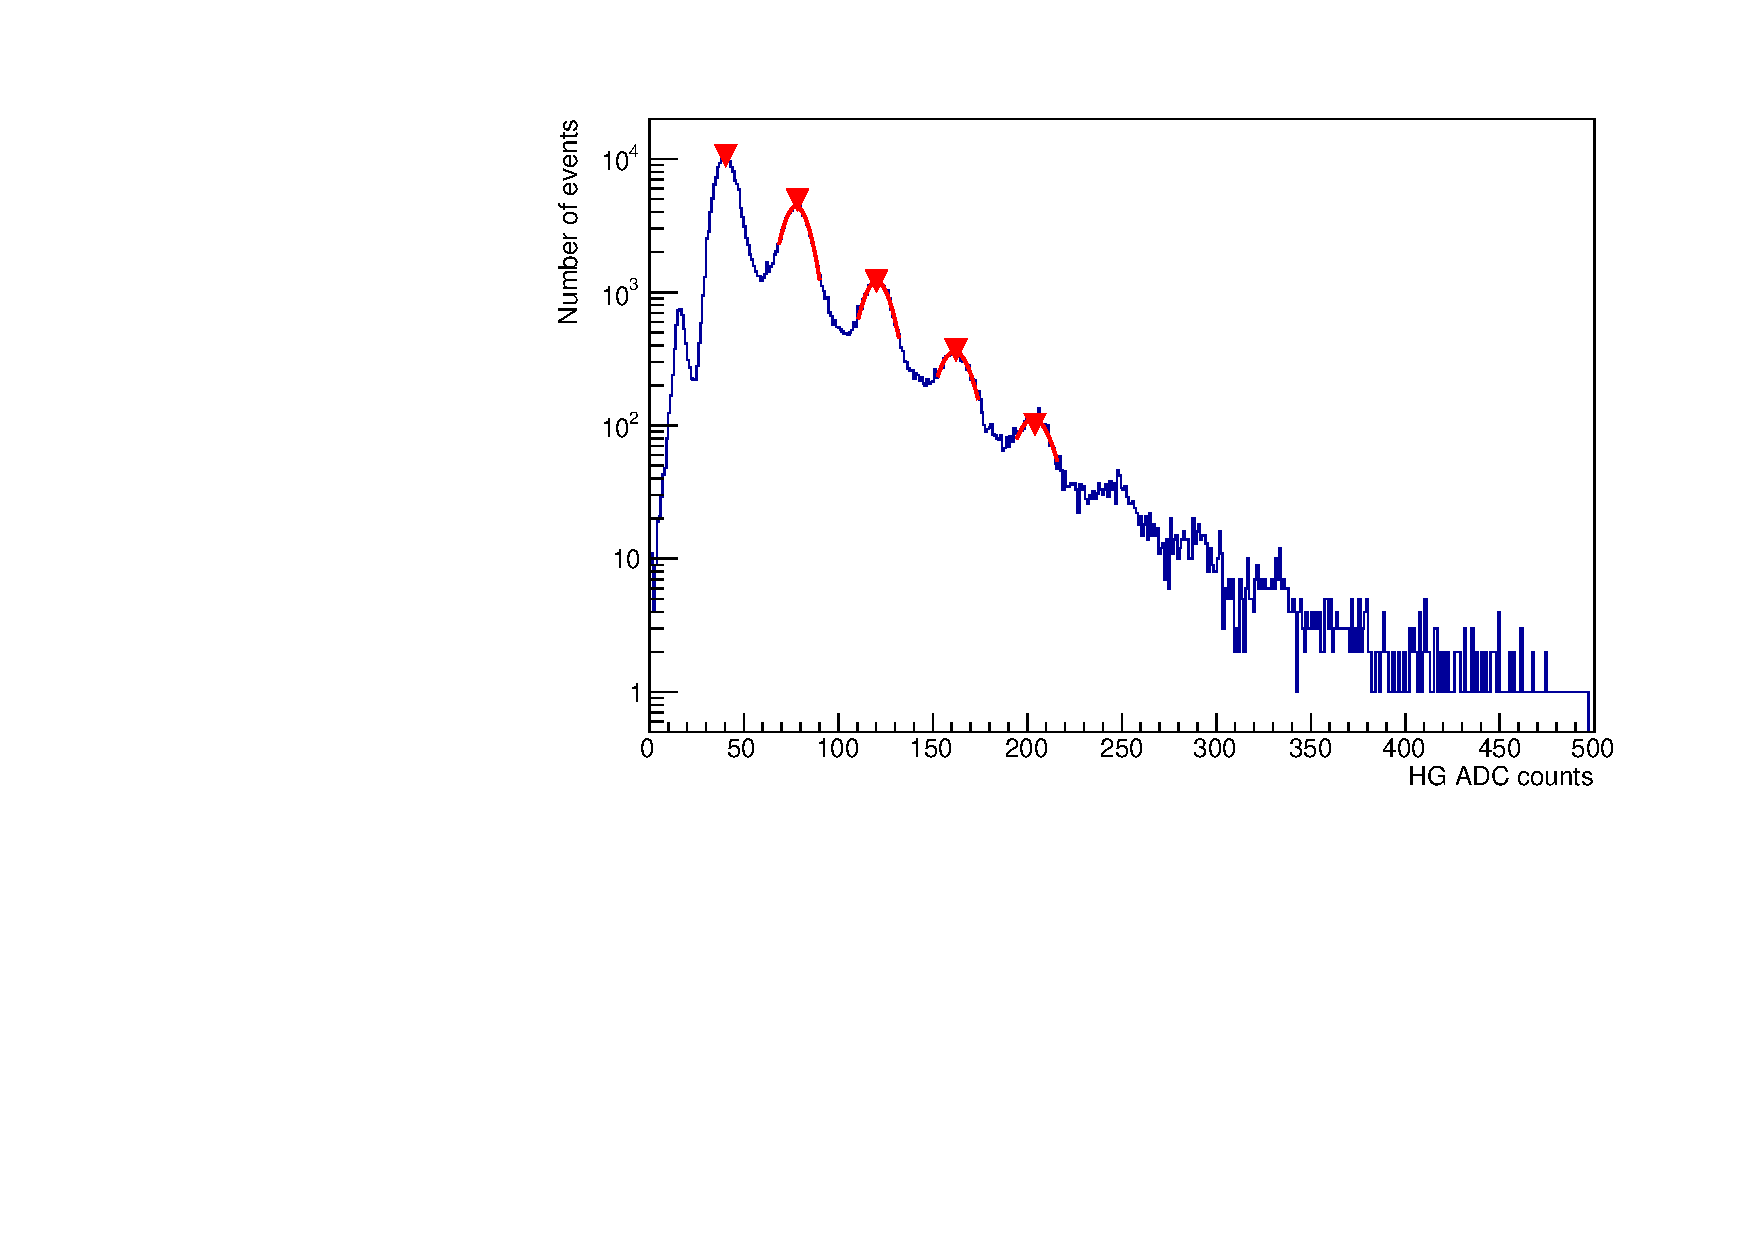
\includegraphics[scale=0.7]{newMPPC}
 \caption{A histogram of the High Gain (HG) analog-to-digital converter (ADC) counts from an MPPC used in the Super-FGD prototype when exposed to low light levels (blue line). The spikes in the data have been fitted with four Gaussian distributions (red lines) in order to calculate the gain of the MPPC. A peak finder was used to find the spikes (red arrows). The peak finder ignored spikes if they were below a certain threshold, and the first peak found by the peak finder was not fitted, as may have been affected by the pedestal signal.}
 \label{fig:mppc}
\end{figure}
shows an example of the signal from an MPPC. The first peak in the plot, with no red arrow, is actually most likely a pedestal peak, which corresponds to zero electrons. The next peak, which is marked with an arrow, may also be affected by this pedestal peak. The following peaks are created purely by photoelectrons incident on the pixels of the MPPC. 
 
The MPPCs used to read off the signal from the Super-FGD need to be calibrated so that the signal can be converted to the total number of photons detected by the photosensor. One of the calibration requirements is to measure the gain of each MPPC, the gain being the factor by which the initial photoelectron's charge is increased by the MPPC. The gain can be calculated by measuring the gaps between peaks in an MPPC's signal. The signal in Fig.~\ref{fig:mppc} has been fitted with four Gaussian distributions to find the centres of the peaks present in its signal, the peaks themselves having been found by a peak finder algorithm. Measuring the distance between these peaks gives a gain of the MPPC of 46.2 $\pm$ 0.5 ADC counts per photoelectron. This measurement needs to be done for all 1728 MPPCs of the Super-FGD detector, which is an ongoing process. Notice that the first peak found by the peak finder was not fitted. This is because this peak is most likely contaminated by the pedestal signal produced by the MPPC, which is not well understood and is normally left out of analyses.

\subsection{Initial Data}
The data collected by the Super-FGD prototype during one of the first test beam runs is shown in Fig.~\ref{fig:hit}.
\begin{figure}
 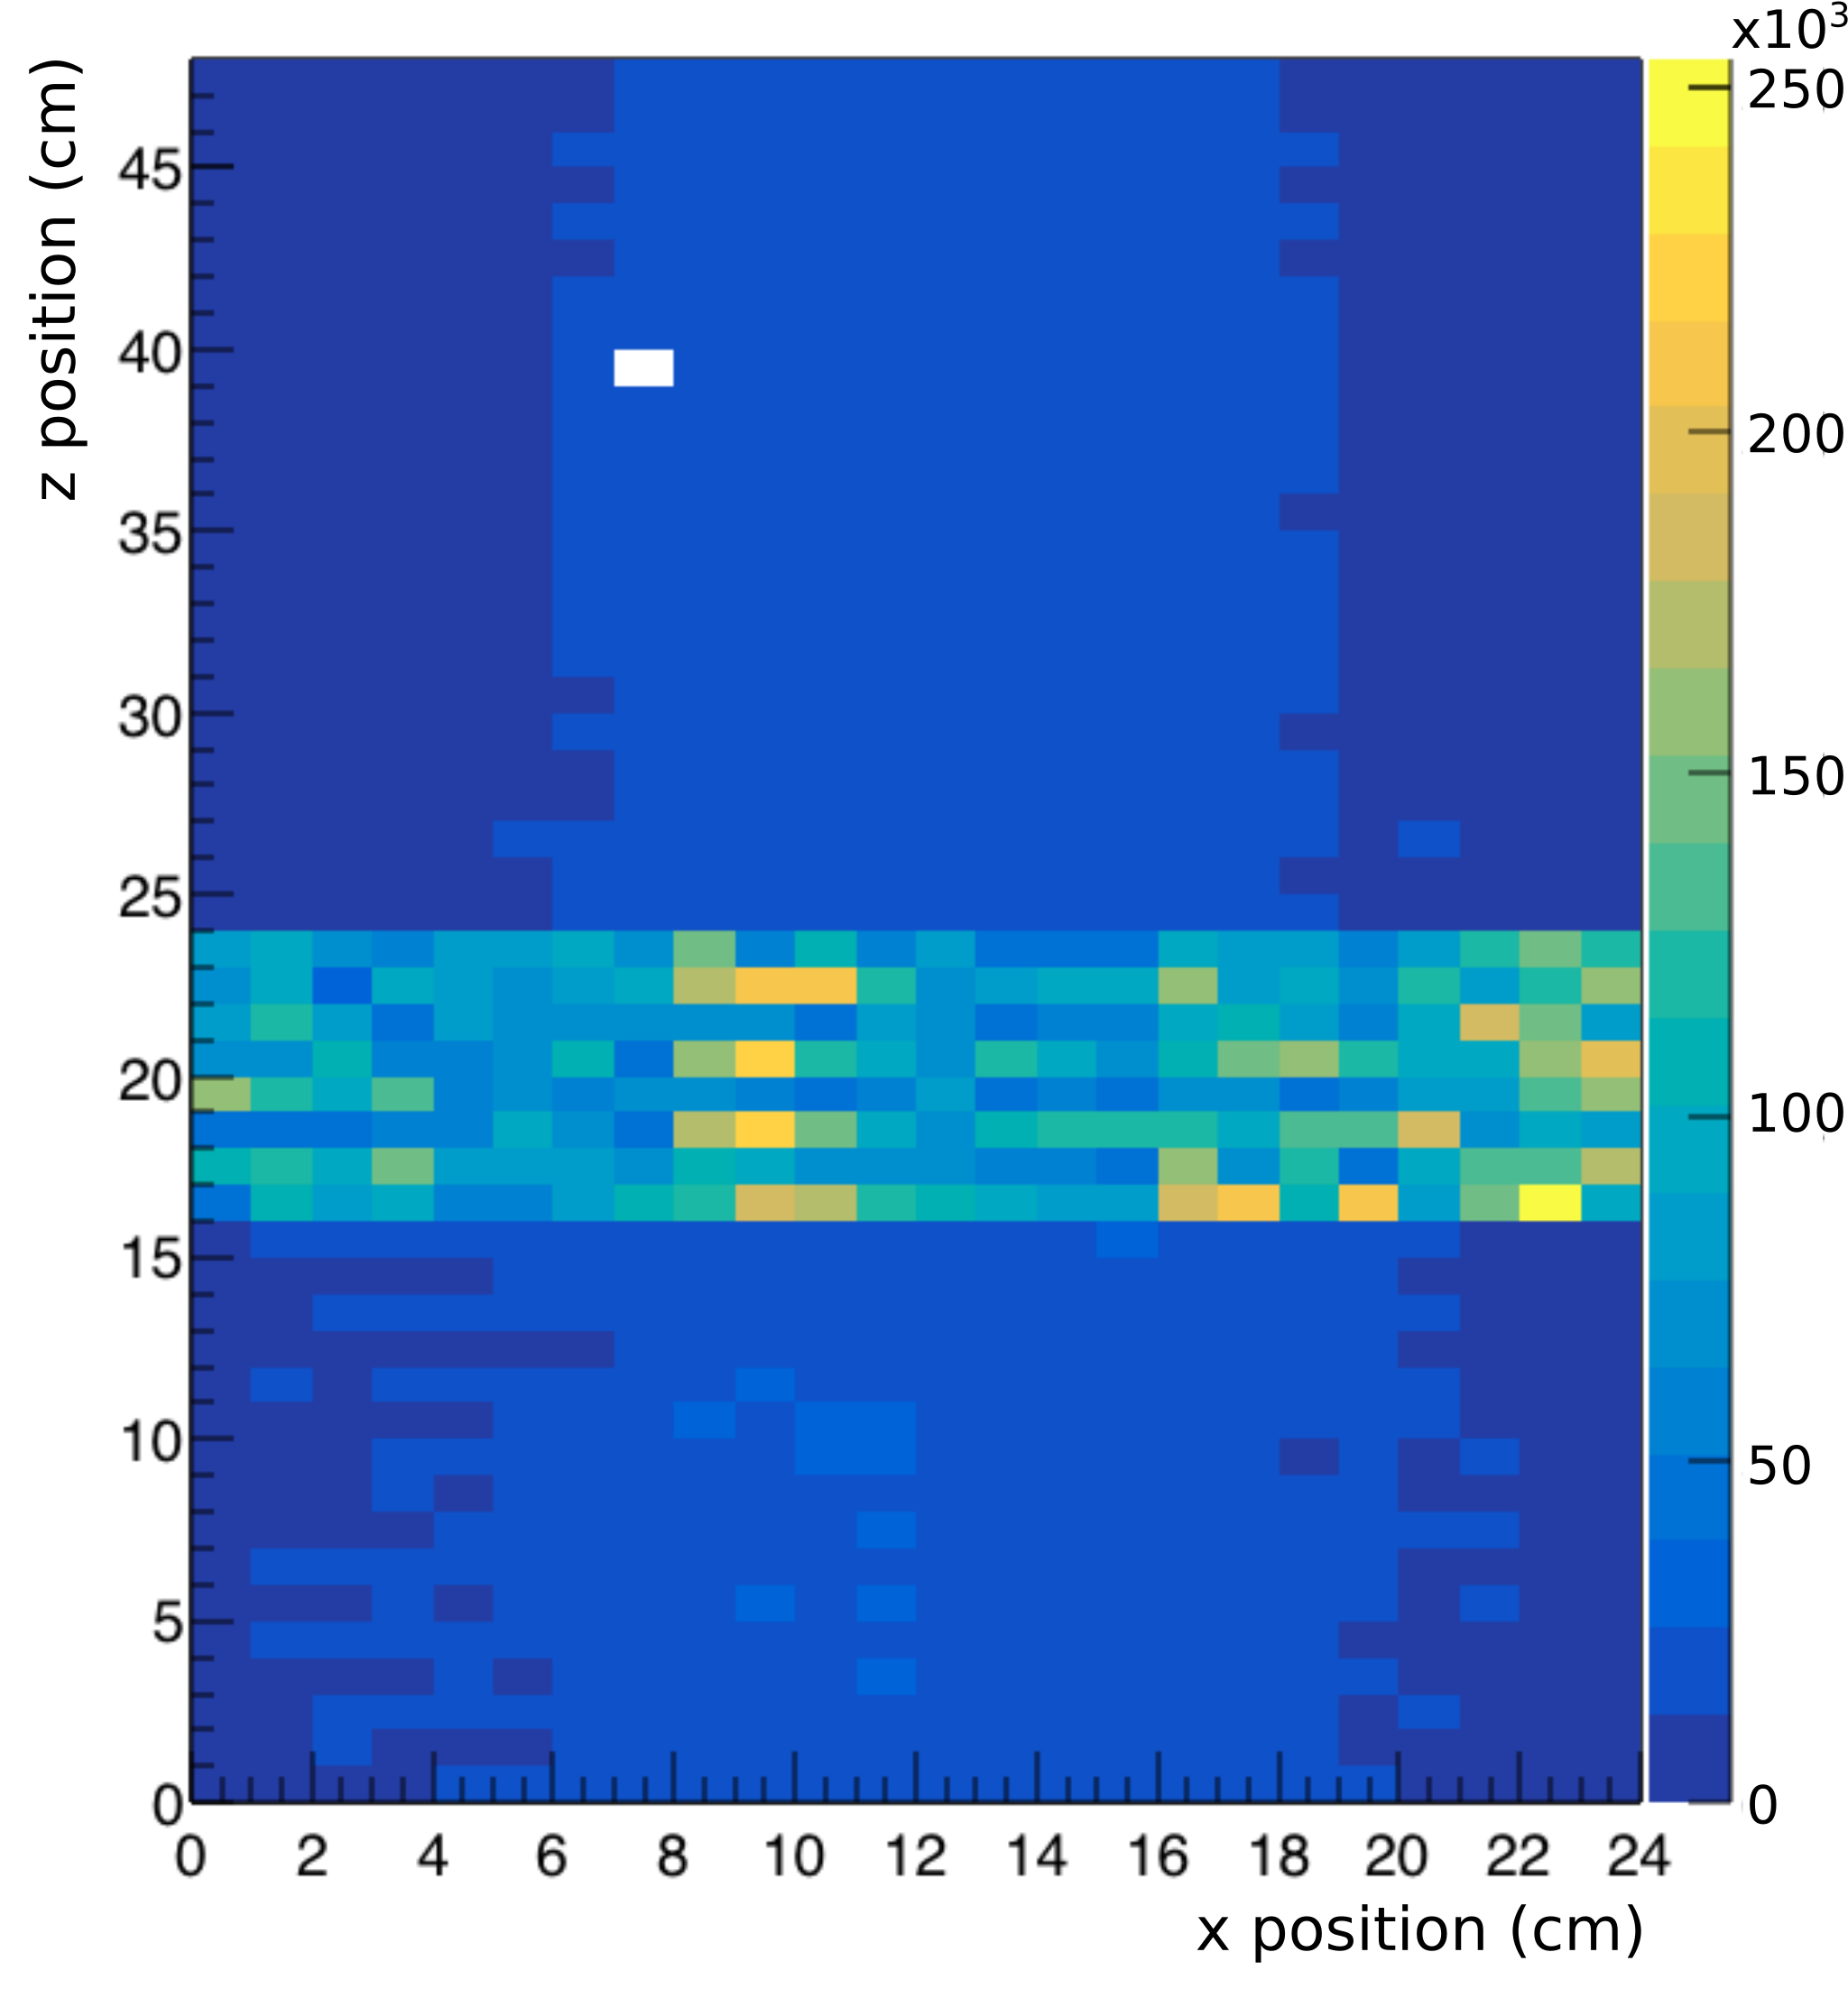
\includegraphics[scale=0.5]{hit_event2}
 \caption{An event map showing the number of events detected by MPPCs on the horizontal faces of the prototype.}
 \label{fig:hit}
\end{figure}
The plot shows the number of signals detected by the MPPCs on the top and bottom of the detector. One can see events corresponding to the particle beam by observing the light blue region running through the centre. There is also a bar of noise along the $x$-axis of the detector. This occurs because the MPPCs here are of a different design to the other regions. In fact, there are three different types of MPPC used on the prototype. The first type correspond to the events shown above the noise bar in the plot. These MPPCs cover the sides and bottom of the detector as well. The region below the bar of noise is another type of MPPC, which explains why the width of the beam seems to be slightly bigger in this region, probably corresponding to cross-talk between scintillator cubes. These two MPPC types are designed to have low noise levels, whereas the MPPC type found in the noisy region is not. This may look problematic, but the figure only shows the number of events, not the amplitude of events. When data is analysed it will be an easy task to filter out the noise from these MPPCs by rejecting signals with small amplitudes. 

The use of several different MPPC types was partly a means to lower the construction costs, as the noisy MPPCs are recycled from the Baby MIND detector, but it also gives an opportunity to test MPPCs with different dynamic ranges and to see which are suitable for the final design.

There is also a noticeable white square in the upper-left region of the event map. This is a faulty MPPC that will be fixed when the prototype is taken out of the magnet for calibration.

Having collected data, it will now be analysed and attempts will be made to reconstruct particle paths. There is no script for an event display written yet, but it is being developed for future use. The plan is to examine data and see if MPPCs that gave a signal at the same point in time can be matched up, which should give the ($x$, $y$, $z$) coordinates of a particle's position.

\section{Software Changes}
%There have been few changes to ND280's software structure since it was conceived 14 years ago, despite many new and upgraded software tools being introduced by developers. The proposal of an upgrade to ND280's hardware has sparked discussions of updates to the software, none of which will include a major overhaul of the framework, but will help streamline the code for the modern day developer. 
%
%One of the changes to be made to the software is the location of the its repositories. These will be moved from CVS to GitLab, a service that is better supported and has better features for software development.
%
%There is also likely to be some changes to package naming conventions. Some packages have names that poorly describe their role in the software, and it would be a good idea to give each package name a prefix that indicates its role in the data flow, i.e. a prefix like "Sim" would show a package is used in simulation of data.
%
%As previously mentioned, ND280's software currently relies on CMT to build its package structure. Since the software's creation, a new tool called CMake has been released that is more efficient than CMake. The software group plans to switch to this build tool to help speed up development.
%
%The software will also be adjusted to incorporate ROOT6 instead of ROOT5, making use of the newly introduced features.

In this section, I will outline the changes that have been proposed following discussions from the ND280 software group, some of which are still subject to certain conditions and may change later on.

\subsection{Version Control}
CVS has been the version control system (VCS) of ND280 since it was first made. Back then, there were few alternatives and CVS seemed most suited to the task. More recently, however, advances have been made in the world of VCSs with the introduction and popularisation of distributed systems. CVS is a centralised system. The difference between centralised and distributed VCSs is that centralised VCSs require a master repository to which developers commit changes, but distributed VCSs allow developers to ``clone'' the software and all its metadata to a repository on their own hard drive. There are several advantages to distributed VCSs, including the ability to commit several changes at once, not requiring all developers of the project to see all the changes you make, and not requiring an internet connection for actions other than pulling and pushing data to other repositories.

Following discussions in the software group, it has been decided that the ND280 software will be moved to GitLab, a centralised VCS. GitLab offers several features that will be useful for scientific code development. The University of Warsaw, Poland, has offered to host the private servers required to store the software on GitLab.

\subsection{Package Names}
The coherent muon to electron transition (COMET) experiment is another experiment situated at J-PARC. It is searching for neutrino-less muon to electron decay. COMET based its software structure on that of ND280~\cite{Wu2017}. In the process of editing the software for their specific use, they updated the package names to make them more consistent and clear. The imminent upgrade could be a good opportunity for ND280's software to follow suit, as there are some arguably confusing names and labelling rules.

A good example of COMET's updated package names is the renaming of the package elecSim to SimDetectorResponse. A developer new to the project would find it hard to discern the role of elecSim in the software (which is to simulate the electronics response of the detector), whereas SimDetectorResponse could not be much clearer. The example also highlights COMET's convention to add a prefix to each package name---such as ``Sim'' or in other cases ``Recon'', ``Calib'' and so on---that indicates where the package will be used in the data flow, i.e. in the simulation, the reconstruction, the calibration or something else. ND280 does this to an extent, but not as consistently, and a suffix is usually used rather than a prefix. 

Some other changes made by COMET were the use of capital letters. In ND280, most package names begin with lower-case lettering, but COMET have made each package begin with an upper-case letter (except packages with the ``oa'' prefix). This is a very basic change but one that arguably makes the names neater and easier to pick out in lists. A change was also made to the lettering of acronyms. For example, the package name ``fgdCalib'' in ND280 was changed to ``CalibFGD''. Again, this is a minor change but it makes the name much clearer and avoids confusion between acronyms and words.

From discussions by the ND280 software group, it seems likely that, when the software is migrated to a new VCS, the package names will be updated in a similar manner to the changes made by COMET, although the decision is not yet concrete.

\subsection{CMake and CMT}
The final applications of a software package need to be built after the software is edited or downloaded for the first time. From a developer's standpoint the performance of the build-tool is critical as they will have to build the software many times. A user of the software should only need to build the software applications once, so they are more concerned with the ease-of-use of the build tool. The creation and hierarchy properties of ND280's packages have so far been managed by CMT. Many other high energy physics experiments have used CMT with their software, but recently they have been switching to CMake~\cite{CMake}. One notable example is LHCb, who, until recently, maintained and used CMT before moving to CMake~\cite{Clemencic2012}.

The advantage in using CMake is that it builds significantly faster than CMT, and is arguably more flexible in its coding. ND280 have decided to switch over to CMake, but whether this will be done after the transition to GitLab or during is still undecided. Currently, a few developers are attempting to build the ND280 software with CMake, and the results of their efforts will influence the decision of when to migrate to CMake.

\subsection{Mix-in Classes}
The software of ND280 currently uses ROOT5, but the latest version is ROOT6. It has been decided to update the software to integrate ROOT6, but in doing so a few things must be changed. The implementation of mix-in classes is the most notable issue. Mix-in classes are used in multiple inheritance, where the properties of several classes can be inherited. However, this is not implemented in ROOT6. The problem can be solved by replacing the implementation of the mix-in classes with C macros, but one would also need to alter the user code that accesses the mix-in classes.

To gauge how big a job this would be, I performed a survey on the software to count the number of times mix-in classes are used (they can be identified by the ``TM'' prefix and ``State'' suffix in their name). The survey also identified the software packages and files each reference to the mix-in class was made in, but here I will only quote the final count of mix-in classes: five classes inherited a mix-in class and the mix-in classes are directly used in the code 50 times. This is relatively infrequent so the transition to ROOT6 shouldn't be significantly delayed by the reimplementation of these classes.

\section{Electron (Anti-)Neutrino Detection at ND280}
A new updated analysis of RHC beam data from ND280 for \nue \ and \anue \ charged current interactions producing no pions (\nue/\anue \ CC-0 $\pi$ for short) is about to be performed. Some electron neutrino contamination is expected in the muon neutrino beam produced at J-PARC, making it imperative to try to measure this at ND280 to reduce systematic errors when finding the number of muon neutrinos converted to electron neutrinos at SK.

Results for the analysis are ongoing. Therefore, in this section, the concepts behind the analysis will be introduced through a description of how cuts can be applied to the data to select \nue \ and \anue \ events. An outline of the my upcoming work on the analysis will then be given in the final section, along with other future projects.

\subsection{Selection Cuts}
The goal of the analysis is to detect electrons (positrons) produced by the weak interaction of a \nue \ (\anue) with a nucleus in the fiducial volume of one of the FGD sub-detectors. There will be a large number of background electrons (positrons) present from interactions of other particles, such as pions undergoing inelastic collisions with atomic electrons, causing them to ionise. These unwanted electrons need to be rejected in the analysis. This is made harder by the relatively small number of electrons (positrons) produced in the \nue \ (\anue) interactions. Also, accurate PID is needed to distinguish the electrons (positrons) from other particles in the detector such as pions (and, in the case of \anue , protons).

For PID and rejection of background electrons (positrons), a number of cuts are applied to the data. For the latest analysis, there were 12 cuts in total. Only a few of these will be outlined in the interest of conciseness. Table \ref{tab:cuts} 
\begin{table}
 \begin{tabular}{|c|m{5cm}|m{9cm}|}
  \hline
  Cut No. & Cut Name & Selection Criteria \\
  \hline\hline
  1 & Quality Cut & Event must have good quality data and be in coincidence with one of the eight proton bunches in the beam\\
  \hline
  2 & TPC Activity & At least one track must go in the TPC \\
  \hline
  3 & FGD Fiducial Volume and TPC Hits & Event must start in the FGD's fiducial volume and the TPC track must have at least 18 hits if the ECal is entered by the track, otherwise 36 TPC hits are required.  \\
  \hline
  4 & Momentum Cut & All events with momenta less than 200 MeV/c are cut. \\
  \hline
  5 & PID in TPC and ECal & Event must pass pull cuts from TPC2 d$E$/d$x$ measurements. Cuts vary depending on whether the selected particle entered the ECal or not. \\
  \hline
  6 & Second TPC PID & Pull cuts from measurements by TPC3 must be passed. \\
  \hline 
  7 & Proton PID & This only applies for the anti-neutrino analysis. A cut on the energy over momentum ($E/p$) value is applied. \\
  \hline
  8 & TPC Veto & The difference in the $z$ position measured in TPC2 of the most energetic track and second most energetic track in an event is calculated and cut if it is less than $-$100~mm. \\
  \hline
  9 & Gamma Invariant Mass & The gamma invariant mass for the selected track and nearby tracks is calculated. If the track pair with the smallest invariant mass gives a value less than 100~MeV/c$^2$ then the event is rejected. \\
  \hline
  10 & P\O D, P\O D Ecal and FGD1 Veto & For FGD1 events, a cut is made if there is any activity in the P\O D or P\O D Ecal.\\
  \hline
  11 & Ecal Veto & The $z$ position of the most upstream Ecal cluster and the most downstream $z$ position of the TPC2 track are compared. Event is rejected if the difference is less than $-$100~mm. \\
  \hline
  12 & FGD2 Shower & Only applied to the anti-electron analysis. Electrons produced in FGD1 often shower in FGD2, but the effect is rarer for protons. Hence, for all tracks in the proton momentum region, if the main track does not enter FGD2, or has more FGD1-TPC2 tracks than FGD2-TPC3 tracks, the event is rejected. Cuts are also made if there are less than two FGD2-TPC3 tracks. \\
  \hline 
 \end{tabular}
 \caption{A list of the cuts applied in the \nue \ and \anue \ analyses.}
 \label{tab:cuts}
\end{table}
contains the complete list. The full descriptions of the cuts can be found in Technical Note 282 by Christodoulou et al.~\cite{Christodoulou2017}.

Of the 12 cuts applied to the data, several ensure the sampled data had enough information for useful analysis. For example, cut 2 was the requirement that at least one track must enter a TPC, which is important for PID. This track must produce at least 18 TPC clusters (a cluster is when the charge signal produced by the ionised electrons in the TPC exceeds the required thresholds and quality criteria) if the track enters the ECal. If instead it does not enter the ECal, 36 clusters are required. The difference here is because the information provided by the ECal makes it much easier to identify the particle as an electron. More detail on the minimum number of TPC clusters can be found in Technical Note 149~\cite{Giganti2013}.

There are also cuts to reduce the background signal. These range from momentum cuts (many background electrons and gammas have momenta below 200~MeV/c) to invariant mass calculations of electron-positron pairs to eliminate gamma backgrounds. PID cuts are also used. For example, selected tracks in events only survive cuts if they have electron, muon and pion pull values ($\delta_e, \ \delta_\mu$ and $\delta_\pi$) that lie within certain ranges. A track's pull corresponding to a certain particle is proportional to the difference between the measured ionisation of the track and the expected ionisation produced by the particle. Hence, in the search for \nue \ and \anue, one wants a near zero value of $\delta_e$ and all other pulls to be far from zero.

Cuts to veto particles originating from outside the detector are also used. Selected tracks must start in the fiducial volume of one of the FGDs and be in coincidence with one of the eight bunches of neutrinos in the beam-line (these bunches are a result of the method of proton acceleration at J-PARC).

The selection of positron tracks from \anue \ interactions is more challenging than finding electron tracks from \nue, as the positrons have the same charge as protons and also have similar energy losses in the TPCs at momenta around 1~GeV~\cite{Giganti2013}. Electrons are easily discerned from protons thanks to the magnetic field in the detector making them curve in opposite directions, but this is not the case for positrons. This means more cuts must be introduced to account for background protons. These cuts look at the ratio between the energy deposited by the particle in the ECal and the momenta of the particles, only letting tracks with ratios above a certain threshold through to the rest of the analysis.

\section{Future Work and Conclusions}
I will now outline how I will progress with my PhD by building upon my initial work and taking advantage of potential research opportunities in the future.

My work on the ND280 software has left many potential avenues of work for me, such as assisting with the transition of the software files from CVS to GitLab. Once the code is transferred it will also need to be maintained. This may include copying anything added to the GitLab repositories to a parallel build of the software kept on CVS, something I could be in charge of. I may also implement a validation system on GitLab that ensures anything uploaded to the software repositories doesn't cause the software to stop functioning.

There is also the switch from CMT to CMake for the software build. This may be done during the transition to GitLab or after. In either case, I will be able to help implement the CMake build with assistance from members of COMET, another J-PARC experiment that is also transitioning their software from CMT to GitLab~\cite{Wu2017}.

I am becoming familiar with the new Super-FGD detector to be installed for the ND280 upgrade thanks to my work on the beam test. This will lead on to me helping with the analysis of the beam test data. From there, I may also become involved with the actual Super-FGD and help to get it ready for installation at ND280.

I will also progress with my work on the updated analysis of \nue \ and \anue \ at ND280 for the RHC beam data. My future work will involve trying to reproduce the selection plots produced in the Production 6 analysis, then I will move on to using the updated MC data and extracting the \nue \ and \anue composition of the beam and the detector's systematic errors by performing fits on the data after selection cuts. 

Looking at more long-term options that will make up the bulk of my thesis, I plan to undertake an analysis/task that combines my recent work on the ND280 upgrade and the electron neutrino contamination analysis at the near detector. One possible path, and one I have set as my main project for the future, is to help with software preparation for the new ND280 detectors, such as implementing the calibration methods, before they are used in ND280 itself. This will make use of the results from the beam tests of the upgraded detectors, which are being carried out this year. For this software preparation, I will be working with Dr.\ Per Jonsson, who is Calibration Convener at ND280. 

There is also the possibility of preparing an analysis for the new detectors. My PhD will end before the detectors are installed and an analysis of their data can be performed, but a Future Analysis Task Force, led by Dr.\ Phillip Litchfield, will provide recommendations for the T2K Collaboration on how future oscillation analyses could proceed. With help from colleagues in one of the main analysis groups---Mach3---I could help implement these analysis preparations, with either the existing detectors or the upgraded detectors.

After joining the T2K group at Imperial College London, I have learnt much about the experiment and gained experience working with software and hardware. Whatever happens over the next few years, there are plenty of exciting options to keep me busy!

%\section{Summary}

\bibliographystyle{mystyle}
\bibliography{bibliography.bib}

\end{document}
